% =====================================================================
% CodeGuard AI - final year project report
% Invertis University, Bareilly - AY 2026-2027
%
% Build:  pdflatex main && bibtex main && pdflatex main && pdflatex main
% or:     latexmk -pdf main.tex
%
% The chapter sources are generated from the Markdown drafts in
% docs/report/ and are overwritten by the build. Edit the Markdown,
% or adopt these .tex files as the source and stop regenerating them -
% but do not edit both, because one of the two will silently win.
% =====================================================================
\documentclass[12pt,a4paper,oneside]{report}

\usepackage[T1]{fontenc}
\usepackage[utf8]{inputenc}
% Guarded: present on MiKTeX and full TeX Live, absent on minimal installs.
% Without it the default Computer Modern is used, which is fine but renders
% as bitmap fonts in some viewers.
\IfFileExists{lmodern.sty}{\usepackage{lmodern}}{}
\usepackage[a4paper,margin=1in,bindingoffset=6mm]{geometry}
\usepackage{graphicx}
\usepackage{longtable,booktabs,array,calc}
\usepackage{caption}
\usepackage{textcomp}
\usepackage{xcolor}
\usepackage{enumitem}
\IfFileExists{microtype.sty}{\usepackage[protrusion=true,expansion=false]{microtype}}{}
\usepackage[numbers,sort&compress]{natbib}
\usepackage{fancyhdr}
\usepackage{mdframed}
\usepackage{comment}
\usepackage[hidelinks,breaklinks]{hyperref}

% ---------------------------------------------------------------------
% Draft notes.
%
% Each chapter carries notes addressed to the author: what still needs
% checking, what is blocked, what must not be submitted as it stands.
% They are NOT part of the report.
%
% Set this to \draftnotesfalse for the submission build and they all
% disappear. Leave it true while the blocked items are outstanding, so
% that a note cannot be submitted by accident.
% ---------------------------------------------------------------------
\newif\ifdraftnotes
\draftnotestrue

\ifdraftnotes
  \definecolor{draftrule}{HTML}{B3261E}
  \definecolor{draftback}{HTML}{FDF3F2}
  \newmdenv[
    linecolor=draftrule, linewidth=1pt,
    backgroundcolor=draftback,
    leftmargin=0pt, rightmargin=0pt,
    innerleftmargin=8pt, innerrightmargin=8pt,
    innertopmargin=6pt, innerbottommargin=6pt,
    skipabove=10pt, skipbelow=10pt,
    frametitle={\textbf{DRAFT NOTE \textendash\ not part of the report}},
    frametitlebackgroundcolor=draftback,
  ]{draftnote}
\else
  \excludecomment{draftnote}
\fi

% pandoc emits \tightlist for compact lists
\providecommand{\tightlist}{%
  \setlength{\itemsep}{0pt}\setlength{\parskip}{0pt}}

\captionsetup{font=small,labelfont=bf}
\setlength{\parskip}{0.4em}
\setlength{\parindent}{0pt}

\pagestyle{fancy}
\fancyhf{}
\fancyhead[L]{\small\nouppercase{\leftmark}}
\fancyhead[R]{\small\thepage}
\renewcommand{\headrulewidth}{0.4pt}

\hypersetup{
  pdftitle={Code Plagiarism Detector Using AST and Behavioural Fingerprinting},
  pdfauthor={Mohd Saqlain Hussain},
}

\begin{document}

% ---------------------------------------------------------------- title
\begin{titlepage}
\centering
\vspace*{1.5cm}

{\LARGE\bfseries Code Plagiarism Detector Using AST\\[0.3em]
and Behavioural Fingerprinting\par}

\vspace{0.8cm}
{\Large CodeGuard AI\par}

\vspace{1.2cm}
{\large A project report submitted in partial fulfilment\\
of the requirements for the degree of\par}
\vspace{0.4cm}
{\large\bfseries Bachelor of Technology\par}
{\large in Computer Science and Engineering\par}

\vspace{1.5cm}
{\large\bfseries Submitted by\par}
\vspace{0.3cm}
{\large Mohd Saqlain Hussain\par}

\vspace{0.4cm}
{\normalsize
Vanshika Uppal \quad\textbullet\quad Trisha \quad\textbullet\quad Shubham\par}

\vspace{1.5cm}
{\large\bfseries Under the guidance of\par}
\vspace{0.3cm}
{\large Mr.\ Ashish Sharma\par}

\vfill
{\large Department of Computer Science and Engineering\par}
{\large Invertis University, Bareilly\par}
\vspace{0.4cm}
{\large Academic Year 2026--2027\par}
\vspace{1cm}
\end{titlepage}

\begin{draftnote}
The title page is a working version. Check it against the department's
prescribed format before submission: roll numbers, the university emblem,
the exact degree wording and the order of names are all things a department
specifies and none of them were available when this was generated. Team
members other than the author are listed without their roles; confirm
whether the department wants them listed at all on a single-author report.
\end{draftnote}

\cleardoublepage
\pagenumbering{roman}
\tableofcontents
\listoffigures
\cleardoublepage
\pagenumbering{arabic}

% -------------------------------------------------------------- chapters
\hypertarget{introduction}{%
\chapter{Introduction}\label{introduction}}

\begin{draftnote}

\textbf{Draft status, 04 November 2026.} \S{}1.4 states the project's
contribution and \textbf{must be settled with the project guide before
submission} --- Chapter 7 \S{}7.9 reports a result that narrows the claim
the project set out with. Chapters 2 \S{}2.7 and 8 \S{}8.6 carry the same flag
and should be settled in one conversation.

\end{draftnote}

\begin{center}\rule{0.5\linewidth}{0.5pt}\end{center}

\hypertarget{the-problem}{%
\section{The problem}\label{the-problem}}

Programming assignments are unusually easy to plagiarise and unusually
hard to check. Source code can be copied and then transformed ---
identifiers renamed, statements reordered, whitespace and comments
rewritten --- until a text-based comparison sees nothing, while the
program remains the same program. A marker reading fifty submissions
cannot hold fifty files in mind well enough to notice that two of them
share a structure, and a marker reading five hundred cannot begin.

There are three distinct problems hiding under the single word
``plagiarism'', and they are not variations of one another:

\textbf{Collusion.} Two or more students submit substantially the same
work. There are at least two copies, and they are both in the cohort.

\textbf{Outsourcing.} A student submits work written by somebody else
--- a paid third party, a senior, a friend outside the course.
\textbf{There is exactly one copy, and the author is not enrolled.}

\textbf{Machine generation.} A student submits work produced by a
language model. Again there is one copy, and again no second copy exists
anywhere to compare against.

Every widely deployed tool addresses only the first. MOSS and JPlag
compare submissions against one another, which is exactly the right
design for collusion and structurally incapable of seeing the other two.
A tool that compares submissions pairwise can detect only collusion,
however good it is at that.

\hypertarget{why-a-single-similarity-percentage-is-the-wrong-output}{%
\section{Why a single similarity percentage is the wrong
output}\label{why-a-single-similarity-percentage-is-the-wrong-output}}

The conventional output of these tools is a similarity figure, and a
conventional institutional practice is to set a threshold on it.

This is wrong in a way that matters, and the clearest statement of why
comes from a systematic review rather than from this project:
\emph{tools do not find plagiarism regardless of how good they are}
\cite{novak2019}. Similarity is not plagiarism. Two students taught the
same algorithm in the same lecture, in a language with strong idioms,
writing a tightly specified exercise, will produce similar code. A
percentage above a threshold is a \emph{judgement} the tool is not
entitled to make, presented in a format that invites it to be acted on
mechanically.

The consequences of acting on it mechanically fall on students, and they
fall hardest on the honest ones, because a flagged honest student has no
second copy to point at in their defence.

\hypertarget{the-approach-an-evidence-system-not-a-verdict-machine}{%
\section{The approach: an evidence system, not a verdict
machine}\label{the-approach-an-evidence-system-not-a-verdict-machine}}

This project's governing principle is that the system produces \textbf{a
ranking with its evidence attached, and a human being decides.}

Concretely, that means:

\begin{itemize}
\tightlist
\item
  the output is an ordering of where a reviewer's attention is best
  spent, not a determination;
\item
  every score carries the evidence that produced it, stored rather than
  recomputed, so it remains readable after the configuration changes;
\item
  where the system cannot tell, it says so, instead of emitting a number
  that looks like an answer;
\item
  a student may see the decision recorded about them and answer it, and
  may not see the score, because a ranking a student can read is a
  ranking a student can tune against.
\end{itemize}

The system asks two questions of a submission, in two layers.
\textbf{Layer 1} asks \emph{does this resemble another submission?},
comparing normalised abstract syntax trees so that renaming and
reordering do not hide a copy. \textbf{Layer 2} asks a different
question, and it is the one the deployed tools cannot ask: \emph{does
this resemble its own author's previous work?} That question needs no
second copy, which is why it is the only route to outsourced work.

A third layer, for machine-generated code, was specified and
\textbf{deliberately not built}; the reasoning is in Chapter 5 \S{}5.4 and
is a requirements argument rather than a scheduling one.

The two layers are composed into a single \textbf{Review Priority
Score}, renormalised over the layers that actually ran, with the weights
and threshold that produced it stored on the result.

\hypertarget{objectives-and-contribution}{%
\section{Objectives and
contribution}\label{objectives-and-contribution}}

The project's objectives were:

\begin{enumerate}
\def\labelenumi{\arabic{enumi}.}
\tightlist
\item
  To build a working system that ingests programming submissions, scores
  them across multiple independent detection layers, and presents a
  ranked review queue with auditable evidence.
\item
  To design and implement behavioural fingerprinting --- per-student
  stylistic baselining --- as a route to detecting work with no second
  copy.
\item
  To protect honest students from the characteristic failure of such a
  system, a wrong baseline, through explicit integrity mitigations.
\item
  \textbf{To measure the result honestly enough to state where it
  fails.}
\end{enumerate}

Objectives 1, 3 and 4 were met. Objective 2 was implemented and then
measured, and the measurement does not support it for partial
outsourcing: Chapter 7 reports that the behavioural layer, as built,
cannot detect a submission that is partly somebody else's, together with
a diagnosis of why and a specific design remedy.

\begin{draftnote}

\textbf{This section is not final.} How the contribution is stated
depends on that result, and the wording is pending a conversation with
the project guide. The defensible position is that the contribution is a
working two-layer evidence system together with a measured negative
result and a diagnosed mechanism --- not a demonstrated capability to
detect outsourced work. Chapters 2 \S{}2.7 and 8 \S{}8.6 must be settled
consistently with whatever is decided here.

\end{draftnote}

\hypertarget{scope}{%
\section{Scope}\label{scope}}

\textbf{In scope.} Single-file submissions in Python and Java; collusion
detection by structural similarity; behavioural baselining per student
per language; configuration per course with per-language overrides; a
reviewer queue and evidence view; a student view and right of reply; an
audit log.

\textbf{Out of scope.} Detection of machine-generated code (Chapter 5
\S{}5.4); multi-file and archive submissions; languages other than Python
and Java; any automated action against a student. \textbf{No output of
this system constitutes a finding of academic misconduct.}

\hypertarget{structure-of-this-report}{%
\section{Structure of this report}\label{structure-of-this-report}}

\begin{longtable}[]{@{}
  >{\raggedright\arraybackslash}p{(\columnwidth - 2\tabcolsep) * \real{0.5000}}
  >{\raggedright\arraybackslash}p{(\columnwidth - 2\tabcolsep) * \real{0.5000}}@{}}
\toprule\noalign{}
\begin{minipage}[b]{\linewidth}\raggedright
chapter
\end{minipage} & \begin{minipage}[b]{\linewidth}\raggedright
contents
\end{minipage} \\
\midrule\noalign{}
\endhead
\bottomrule\noalign{}
\endlastfoot
2 & Literature survey: where the layers come from, and where prior work
stops \\
3 & System analysis and requirements, summarising Appendix A \\
4 & System design: architecture, data flow, data model, the Layer 2
pipeline, score composition \\
5 & Implementation: how each layer works, and why Layer 3 does not
exist \\
6 & Testing and verification, including mutation testing \\
7 & Results and discussion, including the negative result for Layer 2 \\
8 & Conclusion and future work \\
9 & References \\
A & Software Requirements Specification \\
\end{longtable}

\hypertarget{literature-survey}{%
\chapter{Literature Survey}\label{literature-survey}}

\begin{draftnote}

\textbf{Draft status, 03 November 2026.} This prose was written from the
argument and reading notes already recorded in
\texttt{docs/report/chapter2\_plan.md}, which states that every citation
in \texttt{references.bib} was checked against a publisher record or an
author's own copy. \textbf{No factual claim about any paper has been
added here beyond what that plan records.} Two consequences follow, and
both must be dealt with before submission:

\begin{enumerate}
\def\labelenumi{\arabic{enumi}.}
\tightlist
\item
  Nine of the thirteen entries in \texttt{references.bib} still carry a
  TODO on at least one field. Every one is a real publication with a
  confirmed title; each needs a look at the publisher record. Chapter 2
  can be written around them, but the bibliography cannot be printed
  until they are filled.
\item
  The plan's target is 15 to 25 references and the bibliography holds
  13. The seven gaps are named in the plan's own table and restated in
  \S{}2.8 below. Do not pad the count; close the named gaps.
\end{enumerate}

Sections are numbered for a nine-chapter LaTeX report. Citation keys
match \texttt{references.bib}. Replace \texttt{\textbackslash{}cite\{\}}
with the house style if it differs.

\end{draftnote}

\begin{center}\rule{0.5\linewidth}{0.5pt}\end{center}

\hypertarget{what-this-chapter-has-to-establish}{%
\section{What this chapter has to
establish}\label{what-this-chapter-has-to-establish}}

A literature survey in a project report is often a sequence of
summaries. That is not what this chapter is for. Its job is to establish
that the system described in the chapters that follow needed building
--- that the gap it occupies is a real gap in the published work, and
not simply a gap in the author's reading.

The argument runs in four steps, and the chapter is organised around
those steps rather than around chronology. Source-code similarity
detection is a mature field whose best work is explicit that it detects
similarity and not plagiarism. That maturity, however, is confined to
one question: whether two submissions resemble each other. Code
authorship attribution asks a different and more useful question, but
asks it in a form that a university course cannot supply the inputs for.
Detection of machine-generated code exists but depends on training data
that a course cannot supply either. What is missing is not a better
algorithm in any one strand; it is a defensible way of combining them
and reporting the result so that a human being can act on it.

\hypertarget{the-anchoring-result-tools-do-not-find-plagiarism}{%
\section{The anchoring result: tools do not find
plagiarism}\label{the-anchoring-result-tools-do-not-find-plagiarism}}

The most directly relevant published statement of this project's
governing principle is in Novak, Joy and Kermek's systematic review of
source-code similarity detection and the tools used in academia
\cite{novak2019}. Their review concludes that \emph{tools do not find
plagiarism regardless of how good they are}, and that a human must judge
what counts as plagiarism in a given academic context. They identify
JPlag, MOSS and Sherlock Warwick as the most promising of the available
tools, and they report two facts about the field that bear directly on
how this project should be evaluated: most academic tools are never
released, and most are never compared against one another.

This matters more than a design preference being validated. CodeGuard AI
is built as an evidence system rather than a verdict machine: it ranks
submissions for human review and attaches the evidence for its ranking,
and it deliberately does not decide whether plagiarism occurred. Stated
by the author of a project, that is a preference, and it invites the
objection that ranking rather than deciding is a way of avoiding the
hard part of the problem. Stated in \emph{ACM Transactions on Computing
Education} by the authors of a systematic review, it is a position with
support behind it.

It also supplies the justification for the specific output this system
produces. If a tool cannot determine plagiarism, then a single
similarity percentage compared against a threshold is the wrong
interface, because it presents a judgement the tool is not entitled to
make. A ranked score with its evidence attached presents what the tool
actually has: an ordering of where a reviewer's attention is best spent.

\hypertarget{token-and-fingerprint-methods-and-the-question-they-cannot-ask}{%
\section{Token and fingerprint methods, and the question they cannot
ask}\label{token-and-fingerprint-methods-and-the-question-they-cannot-ask}}

The dominant family of deployed tools compares submissions as sequences
of tokens. Schleimer, Wilkerson and Aiken's winnowing algorithm
\cite{schleimer2003} is the fingerprinting scheme behind MOSS. Winnowing
selects the minimum hash from each window of consecutive k-gram hashes,
which yields a guarantee that any shared substring of length at least
\texttt{w\ +\ k\ -\ 1} produces at least one matching fingerprint. That
guarantee is the reason MOSS both works and scales: the index is a small
fraction of the corpus, and the matching property is provable rather
than empirical.

JPlag \cite{prechelt2002} takes a different route to the same question.
It tokenises each submission using a language-aware front end, so that
identifier names and formatting are discarded before comparison, and
then runs greedy string tiling over the resulting token streams to find
maximal matching segments.

Both are strong, mature, and widely used. Both also share a structural
limitation, and it is this limitation that opens the space the present
project occupies: \textbf{they compare submissions against each other.}
They are built to answer the question \emph{did two students hand in the
same work?} Consequently there are three forms of academic misconduct
they cannot see at all:

\begin{itemize}
\tightlist
\item
  work outsourced to a paid third party, where no second copy exists
  anywhere in the cohort;
\item
  work generated by a language model, for the same reason;
\item
  work taken from a previous year's cohort, unless that corpus has been
  retained and is included in the comparison set.
\end{itemize}

A tool that compares submissions pairwise can detect collusion and
nothing else. Collusion is real and is the most common case, which is
why these tools remain valuable. But it is one of the three threats
named in this project's scope, and the other two require a different
question to be asked of a submission: not \emph{does this resemble
another submission?} but \emph{does this resemble its own author?}

\hypertarget{tree-and-ast-methods-layer-1s-ancestry}{%
\section{Tree and AST methods: Layer 1's
ancestry}\label{tree-and-ast-methods-layer-1s-ancestry}}

Moving from token streams to syntax trees is what buys resistance to the
obfuscations a student actually applies. Renaming identifiers,
reordering independent statements and reformatting whitespace all change
the token stream while leaving the abstract syntax tree largely intact,
because an AST discards precisely the surface detail those
transformations alter.

The algorithm this project's structural layer calls directly is APTED,
from Pawlik and Augsten \cite{pawlik2016}. Their earlier RTED paper
\cite{pawlik2015} establishes the dynamic decomposition strategy that
the later work builds on, and the authors ask that both be cited
together; this report does so. DECKARD \cite{jiang2007} takes the
alternative path: rather than computing an edit distance between trees,
it characterises subtrees as numerical count vectors and clusters them
using locality-sensitive hashing, trading exactness for scale. The
distinction is worth stating explicitly in a report whose own Layer 1
chooses exactness and then prefilters to recover scale, which is a
hybrid of the two positions.

Zakeri-Nasrabadi et al.'s systematic review \cite{zakeri2023} supplies
the taxonomy within which Layer 1 can be located: text, token, tree,
graph, metric, learning, image and test-based approaches, with hybrids
the most common category at approximately 28\% of the studies surveyed.
Two of their findings should be carried into this report rather than
discovered under questioning.

First, \textbf{Type IV (semantic) clones remain hard, and many
techniques cannot detect them at all.} Layer 1 shares that limitation.
Two implementations of the same algorithm with different structure will
not be matched by tree edit distance, and the report should say so in
its limitations rather than imply a generality the method does not have.

Second, their observation that close to half of surveyed tools support
Java while many languages have little or no support is the cleanest
available justification for this project measuring both Java and Python
separately instead of asserting language portability. The measurements
in Chapter 7 report the two languages apart from each other for exactly
this reason.

\hypertarget{authorship-attribution-layer-2s-ancestry-and-its-trap}{%
\section{Authorship attribution: Layer 2's ancestry, and its
trap}\label{authorship-attribution-layer-2s-ancestry-and-its-trap}}

Code stylometry asks who wrote a file from its style alone.
Caliskan-Islam et al.~\cite{caliskan2015} is the canonical result,
reporting roughly 94\% accuracy across 1,600 programmers and 98\% across
250, using lexical, layout and AST-derived features on Google Code Jam
submissions. Frantzeskou et al.'s SCAP method \cite{frantzeskou2006}
reaches comparable accuracy from byte-level n-gram author profiles
without parsing the source at all. Abuhamad et al. \cite{abuhamad2019}
extend the task to large author populations using deep feature learning.

This is Layer 2's intellectual ancestry, and it is also the single most
dangerous body of work for this project to be measured against. An
examiner who has read Caliskan-Islam will ask why this project reports a
lift of roughly \textbf{1.4x to 2.5x over chance} where the literature
reports \textbf{94\% accuracy}. The question sounds damning. The answer
is not, and it belongs here in Chapter 2 rather than being offered
defensively in Chapter 7 after the numbers have already been presented.

\textbf{The task is not the same one.} The attribution literature
performs closed-set identification: given a file and a known list of N
candidate authors, select the author. Layer 2 performs anomaly detection
against a single reference: given a file and this student's own earlier
work, is it consistent with that work? There is no candidate list, and
there cannot be one, because the ghostwriter is not enrolled in the
course. The two tasks share features and share nothing else.

\textbf{The feature budget is not the same.} Those systems use hundreds
to thousands of features, including deep AST-derived ones. The scoring
in this project uses four, for two reasons: four is what survived
measurement on real code, and every feature contributing to a flag must
be explainable to a student who contests it. A feature a reviewer cannot
explain is not evidence, whatever it contributes to an accuracy figure.

\textbf{The data is not the same.} Google Code Jam provides many authors
solving \emph{identical} problems, which holds the task constant and
allows style to dominate the signal. Coursework has the same property,
which makes it the fair comparison. The figures this project reports,
however, come from library code across 26 open-source repositories,
where the project's own conventions act as a confound; the honest
within-project figures are the lower ones, and Chapter 7 reports them as
such.

\textbf{The success criterion is not the same.} Attribution is graded on
selecting the correct author. Layer 2 is graded on whether a human
reviewer, shown the evidence, reaches a defensible decision. A 2x lift
that surfaces the right twenty submissions out of five hundred is useful
to a marker. A 94\% attribution accuracy over a candidate set that does
not contain the actual author is not a useful number at all.

Positioning the project against this literature before presenting
results is considerably stronger than defending the gap afterwards, and
this chapter should do so explicitly.

\hypertarget{detection-of-machine-generated-code-and-why-layer-3-was-dropped}{%
\section{Detection of machine-generated code, and why Layer 3 was
dropped}\label{detection-of-machine-generated-code-and-why-layer-3-was-dropped}}

The fourth strand is the newest. Nguyen et al.~\cite{nguyen2023}, with
the journal version appearing as GPTSniffer \cite{gptsniffer2024},
fine-tune CodeBERT to distinguish human-written from ChatGPT-written
code, and report outperforming GPTZero and OpenAI's own text classifier
on that task. Two of their findings are directly relevant: performance
improves when the training data resembles the target code, and it
improves when snippets are classified in pairs rather than individually.

\textbf{The first of those findings is the argument for dropping this
project's third layer, and the report presents it as a decision rather
than as an omission.} A classifier whose accuracy depends on its
training data resembling the target requires a labelled corpus of
student work drawn from the course it will police. No such corpus exists
for this project, and none can be manufactured honestly: generating one
would mean producing synthetic ``AI-written'' student submissions and
treating the result as ground truth.

Without that corpus the layer could still be implemented, but its
performance could never be reported. In a system whose entire premise is
auditable evidence, a layer that produces a number nobody can
characterise is worse than a layer that is absent, because a reviewer
has no basis on which to weigh it. The architecture therefore records
the layer's absence explicitly rather than silently omitting it ---
every detection result stores
\texttt{aiContent:\ \{\ status:\ "skipped",\ reason:\ "Layer\ 3\ is\ not\ implemented\ yet"\ \}}
--- and Chapter 8 lists the layer as future work with the labelled
corpus named as its precondition.

This has a consequence for the score composition that Chapter 4
describes in detail and that is worth flagging here: because the third
layer never runs, the configured weights are renormalised over the
layers that did run, and the headline weights are therefore never the
applied ones.

\hypertarget{the-gap-this-project-occupies}{%
\section{The gap this project
occupies}\label{the-gap-this-project-occupies}}

Drawing the four strands together.

Similarity detection is mature, and the best of it is honest about what
it does: it finds similarity, not plagiarism, and a human decides
\cite{novak2019}. But similarity detection can only see collusion,
because it compares submissions against one another
\cite{schleimer2003, prechelt2002}. Tree-based methods make that
comparison robust to the obfuscations students actually apply
\cite{pawlik2016, jiang2007}, which is a genuine improvement, but it
does not change the question being asked. Authorship attribution asks a
question that could in principle see outsourced work, and asks it well
\cite{caliskan2015, frantzeskou2006, abuhamad2019} --- but it is posed
as closed-set identification against a candidate list, and a course does
not have one. Detection of machine-generated code exists, and its
accuracy depends on in-distribution training data that a course does not
have either \cite{gptsniffer2024}.

The contribution claimed by this project is therefore not a better
algorithm in any one of these strands. It is the combination of
structural similarity with per-student stylistic baselining, composed
into a single ranked and auditable figure with its evidence attached,
measured honestly enough to state where it fails.

That is a defensible contribution for a final-year project, and it is
defensible precisely because it does not claim to beat Caliskan-Islam et
al.~at their own task.

\begin{draftnote}

\textbf{Required revision before submission.} The claim in the paragraph
above is stated as the project's contribution. The measurement reported
in Chapter 7 does not support the stylistic-baselining half of it on the
one corpus built to test it: on 214 spliced pairs the behavioural layer
did not detect partial outsourcing, and the mechanism for that failure
is now understood. \textbf{The wording of this project's claimed novelty
therefore has to be settled with the project guide before this section
is finalised}, and Chapter 7 must be written first. Do not submit \S{}2.7
in its present form.

\end{draftnote}

\hypertarget{limitations-of-this-survey}{%
\section{Limitations of this survey}\label{limitations-of-this-survey}}

Stating these is better than leaving an examiner to find them.

\textbf{Coverage.} The bibliography holds 13 entries against a target of
15 to 25. The gaps are specific rather than general, and each is wanted
for a stated purpose:

\begin{longtable}[]{@{}
  >{\raggedright\arraybackslash}p{(\columnwidth - 2\tabcolsep) * \real{0.5000}}
  >{\raggedright\arraybackslash}p{(\columnwidth - 2\tabcolsep) * \real{0.5000}}@{}}
\toprule\noalign{}
\begin{minipage}[b]{\linewidth}\raggedright
missing
\end{minipage} & \begin{minipage}[b]{\linewidth}\raggedright
wanted for
\end{minipage} \\
\midrule\noalign{}
\endhead
\bottomrule\noalign{}
\endlastfoot
Baxter et al., clone detection using ASTs, ICSM 1998 & the origin of
AST-based clone detection; Layer 1's grandparent \\
Joy and Luck, plagiarism in programming assignments & the
lexical/structural obfuscation taxonomy \cite{novak2019} draws on \\
CCFinder (Kamiya et al.) & the token-based industrial counterpoint to
DECKARD \\
a study of student plagiarism behaviour & Chapter 1 needs evidence that
the problem is real and common, not assumed \\
Sherlock (Warwick) & named in \cite{novak2019}'s top three; worth a
paragraph \\
contract cheating / essay mills & the outsourcing threat model Layer 2
exists to address \\
a reference for one-way ANOVA and the F ratio & Chapter 7's method needs
a citation, not only an explanation \\
\end{longtable}

Baxter et al.~could not be verified at the time of the original search
and \textbf{must not be cited until it has been}.

\textbf{Verification state.} Four entries have every field confirmed
(\texttt{novak2019}, \texttt{prechelt2002}, \texttt{caliskan2015},
\texttt{nguyen2023}). The remaining nine are real publications with
confirmed titles and at least one unconfirmed field. During the first
drafting of the bibliography three fields were written from memory
rather than read from a source --- a DOI on \texttt{schleimer2003} and
the author lists on \texttt{frantzeskou2006} and \texttt{abuhamad2019}
--- and were removed on a second pass. That is recorded because the
bibliography's own header forbids exactly that practice, and the rule
only caught the error because the file was audited after being written.

\textbf{Depth.} This survey positions the project against prior work; it
does not reproduce or re-implement any of it. No claim in this chapter
rests on a comparison this project ran. Where the report compares its
own figures against published ones, as in \S{}2.5, the comparison is of
\emph{tasks} and not of results, and is argued rather than measured.

\hypertarget{system-analysis-and-requirements}{%
\chapter{System Analysis and
Requirements}\label{system-analysis-and-requirements}}

\begin{draftnote}

\textbf{Draft status, 04 November 2026.} This chapter is the narrative
summary; the full specification is Appendix A
(\texttt{docs/report/SRS.md}), which carries every requirement with a
stable identifier. Requirement numbers used here refer to that document
--- do not renumber them, because Chapter 6's verification refers to the
same identifiers.

\end{draftnote}

\begin{center}\rule{0.5\linewidth}{0.5pt}\end{center}

\hypertarget{the-problem-stated-as-a-requirement}{%
\section{The problem, stated as a
requirement}\label{the-problem-stated-as-a-requirement}}

A member of faculty marking fifty or five hundred programming
submissions needs to know \textbf{where to spend attention}. They do not
need a verdict, and a tool is not entitled to give one (Chapter 2 \S{}2.2).
What they need is an ordering, and a reason for the ordering they can
read, defend to a student, and be held to.

That reframing drives nearly every requirement that follows. The
system's output is a \textbf{ranking with attached evidence}, not a
percentage with a threshold.

\hypertarget{existing-systems-and-where-they-stop}{%
\section{Existing systems, and where they
stop}\label{existing-systems-and-where-they-stop}}

\begin{longtable}[]{@{}
  >{\raggedright\arraybackslash}p{(\columnwidth - 6\tabcolsep) * \real{0.2500}}
  >{\raggedright\arraybackslash}p{(\columnwidth - 6\tabcolsep) * \real{0.2500}}
  >{\raggedright\arraybackslash}p{(\columnwidth - 6\tabcolsep) * \real{0.2500}}
  >{\raggedright\arraybackslash}p{(\columnwidth - 6\tabcolsep) * \real{0.2500}}@{}}
\toprule\noalign{}
\begin{minipage}[b]{\linewidth}\raggedright
system
\end{minipage} & \begin{minipage}[b]{\linewidth}\raggedright
approach
\end{minipage} & \begin{minipage}[b]{\linewidth}\raggedright
what it finds
\end{minipage} & \begin{minipage}[b]{\linewidth}\raggedright
what it cannot find
\end{minipage} \\
\midrule\noalign{}
\endhead
\bottomrule\noalign{}
\endlastfoot
MOSS & winnowing fingerprints over k-grams & submissions resembling each
other & anything with no second copy in the corpus \\
JPlag & language-aware tokenising, greedy string tiling & the same & the
same \\
Turnitin and similar & text similarity against a web and paper corpus &
copied prose, some copied code & code transformed by renaming or
reordering \\
\end{longtable}

All of the above compare submissions \textbf{against each other}. That
is sufficient for collusion, which is the most common case, and
structurally incapable of detecting work outsourced to a third party or
generated by a model, because neither leaves a second copy in the
cohort.

\textbf{The proposed system differs in asking a second question}: not
\emph{does this resemble another submission?} but \emph{does this
resemble its own author's previous work?} Chapter 7 reports the extent
to which the implemented answer to that second question succeeds, and it
is more limited than the design intended.

\hypertarget{user-classes}{%
\section{User classes}\label{user-classes}}

\begin{longtable}[]{@{}
  >{\raggedright\arraybackslash}p{(\columnwidth - 2\tabcolsep) * \real{0.5000}}
  >{\raggedright\arraybackslash}p{(\columnwidth - 2\tabcolsep) * \real{0.5000}}@{}}
\toprule\noalign{}
\begin{minipage}[b]{\linewidth}\raggedright
class
\end{minipage} & \begin{minipage}[b]{\linewidth}\raggedright
may
\end{minipage} \\
\midrule\noalign{}
\endhead
\bottomrule\noalign{}
\endlastfoot
\textbf{Student} & submit work; see their own status and any recorded
decision; answer a flag; nominate past work as an anchor \\
\textbf{Faculty} & create courses and assignments; enrol students; see
the ranked queue and full evidence; record decisions; accept
nominations; re-run detection \\
\textbf{Admin} & all of the above, plus create accounts with roles and
edit detection configuration \\
\end{longtable}

\textbf{A student never sees a score.} This is a requirement (FR-30),
not an oversight: a ranking a student can read is a ranking a student
can tune against. The endpoint backing the student view returns no score
at all, so the property is enforced by the API rather than by the
interface choosing not to display it.

\hypertarget{functional-requirements-in-summary}{%
\section{Functional requirements, in
summary}\label{functional-requirements-in-summary}}

Thirty-two functional requirements, grouped. The full statements are in
Appendix A.

\begin{itemize}
\tightlist
\item
  \textbf{Authentication and accounts (FR-1 to FR-6).} Public
  self-registration creates a student account and no other; role
  assignment is an admin operation.
\item
  \textbf{Courses, enrolment, configuration (FR-7 to FR-10).} Detection
  configuration is per course, with per-language overrides --- because
  the evidence in Chapter 7 \S{}7.4 shows the same feature behaving
  oppositely in Python and Java, a single configuration for both cannot
  be correct.
\item
  \textbf{Assignments (FR-11, FR-12).} An assignment carries its
  language and its provenance, invigilated or take-home, because
  provenance determines whether the work may later serve as a style
  anchor.
\item
  \textbf{Submission (FR-13 to FR-16).} One source file,
  extension-checked and size-limited, stored with a content hash, with
  detection enqueued and debounced rather than run inline.
\item
  \textbf{Detection (FR-17 to FR-22).} Both layers computed where
  possible, composed with renormalisation, with the applied weights, the
  threshold and both layers' \textbf{evidence} stored on the result.
\item
  \textbf{Baseline integrity (FR-23 to FR-28).} The five mitigations
  described in Chapter 4 \S{}4.6.
\item
  \textbf{Review and the student view (FR-29 to FR-31).}
\item
  \textbf{Audit (FR-32).} Every state change affecting a student's
  record, held in a log separate from the documents it describes.
\end{itemize}

\hypertarget{non-functional-requirements}{%
\section{Non-functional
requirements}\label{non-functional-requirements}}

Ten, of which three are worth naming here.

\textbf{Bounded comparison (NFR-3).} The detector accepts at most 50
candidates and compares at most 10 in full, selected by a cheap
prefilter. This bounds the cost of one analysis irrespective of class
size --- and it is also a constraint on \emph{measurement}: a study that
compares exhaustively is measuring a system that was never deployed.
That error was made and corrected (Chapter 7 \S{}7.2).

\textbf{Explainability (NFR-8).} Every feature contributing to a
behavioural score must be explainable to a student contesting a flag.
This is why four features are scored rather than the ten extracted, and
it is a genuine constraint on accuracy: a feature a reviewer cannot
explain is not evidence, whatever it contributes to a score.

\textbf{Stated limitations (NFR-9, NFR-10).} Two requirements in the
specification record what the system does \emph{not} establish --- Layer
2's efficacy against partial outsourcing, and Layer 1's precision and
recall on genuine plagiarism. Recording a limitation as a numbered
requirement is unusual, and it is deliberate: it makes the gap traceable
rather than something a reader must infer from an absence.

\hypertarget{feasibility}{%
\section{Feasibility}\label{feasibility}}

\textbf{Technical.} The parsing and tree-comparison libraries required
are mature and freely available; the architecture is conventional. The
one genuine technical risk was the cost of tree edit distance, and it is
addressed by the prefilter.

\textbf{Operational.} The system requires something a course may not
have: \textbf{attributable past work for each student.} Layer 2 cannot
function without at least three trustworthy anchors per student per
language, and where those do not exist the layer declines to score
rather than guessing. A course with no invigilated work and no
nomination process gets a one-layer system.

\textbf{Ethical.} The system ranks students for suspicion, which carries
a direct risk of harm to an honest student through a wrong baseline.
That risk is the reason for the five mitigations, for the requirement
that a student may answer a flag, for the separate audit log, and for
the decision that no output of this system constitutes a finding of
misconduct.

\textbf{Scope.} Layer 3 was excluded on requirements grounds rather than
schedule grounds, and the reasoning is in Chapter 5 \S{}5.4.

\hypertarget{verification-approach}{%
\section{Verification approach}\label{verification-approach}}

Requirements are verified by the 278-test suite described in Chapter 6,
with identifiers traceable from Appendix A to test cases. NFR-9 and
NFR-10 are verified \textbf{as limitations rather than as capabilities},
by the committed measurement scripts reported in Chapter 7 --- which is
the only honest way to verify a requirement that records what the system
cannot do.

\hypertarget{system-design}{%
\chapter{System Design}\label{system-design}}

\begin{draftnote}

\textbf{Draft status, 04 November 2026.} The five figures referenced
here are committed in \texttt{docs/diagrams/} as Mermaid sources with
rendered \texttt{.svg} (vector, for LaTeX) and \texttt{.png} at 2\texttimes{} (for
slides). Each has a regenerable source beside it, so no figure in this
report is one nobody can reproduce --- the same rule the measurements
folder works under. \textbf{These are the figures the viva will be
conducted from}, so they are worth knowing better than this chapter's
prose.

\end{draftnote}

\begin{center}\rule{0.5\linewidth}{0.5pt}\end{center}

\hypertarget{architecture}{%
\section{Architecture}\label{architecture}}

\begin{figure}[htbp]
\centering
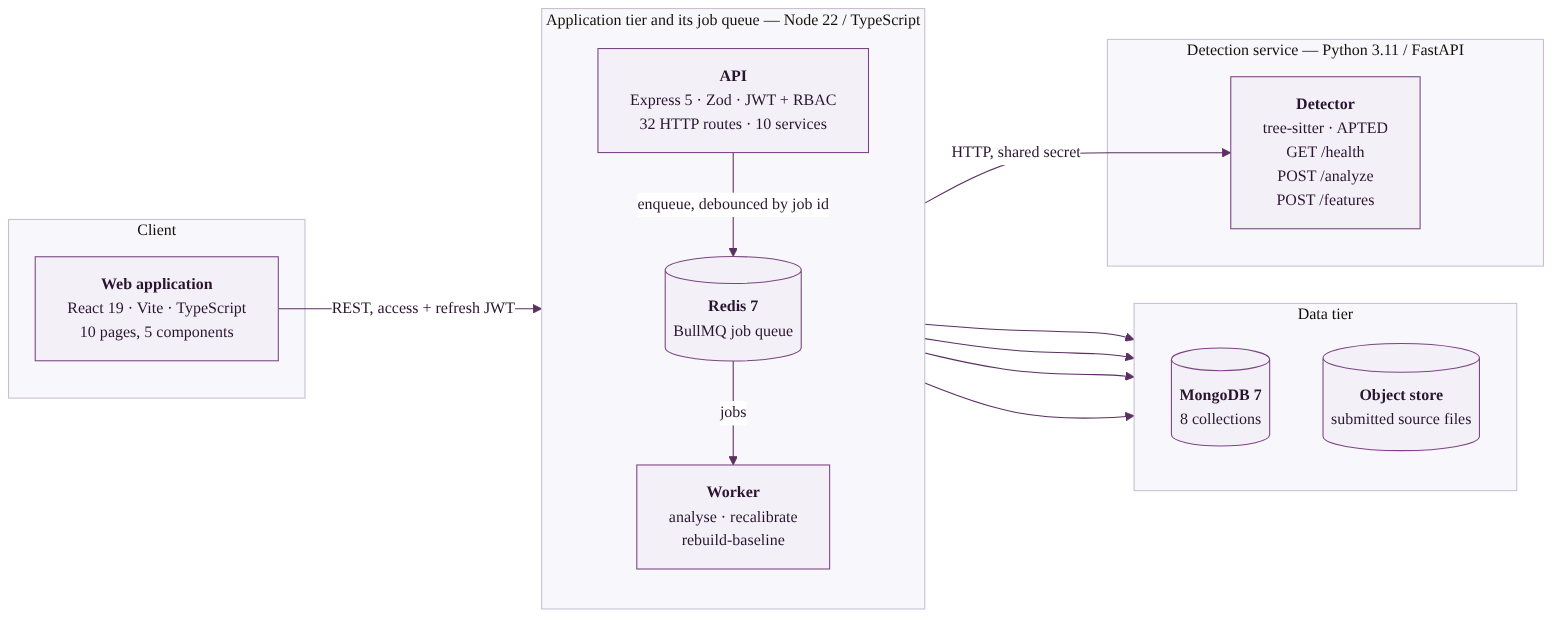
\includegraphics[width=\linewidth,height=0.78\textheight,keepaspectratio]{figures/01-architecture.png}
\caption{System architecture: three tiers and one detection service. The web application never talks to the detector or to any data store; everything goes through the API, which holds the only credentials.}
\label{fig:01-architecture}
\end{figure}

Three tiers and one detection service.

\textbf{The web application never talks to the detector or to any data
store.} Everything goes through the API, which holds the only
credentials in the system. That is the single most important property of
the diagram and the one to point at first: there is exactly one tier
where a credential exists, exactly one tier that can reach MongoDB,
Redis or the object store, and exactly one place where an authorisation
decision is made.

Redis is drawn inside the application tier to keep the queue flow
legible, but it is infrastructure and runs as its own container
alongside MongoDB and the object store.

\textbf{The worker is the same codebase as the API, started on a
different entry point.} A queued job and a synchronous request therefore
share one set of services rather than two implementations that can drift
apart. Two copies of the scoring logic would eventually disagree, and
the disagreement would surface as a result nobody could reproduce.

The split between the API and the detector deserves defending, because
it looks like unnecessary complexity for a student project. It is not.
The parsing ecosystem this system depends on --- tree-sitter grammars
and an APTED implementation --- is Python. The web application and its
document model are far more naturally written in TypeScript against
Mongoose. Rather than compromise one to accommodate the other, the
detector is a \textbf{stateless} HTTP service that parses and compares,
and every piece of state stays in the API.

\hypertarget{one-submission-end-to-end}{%
\section{One submission, end to end}\label{one-submission-end-to-end}}

\begin{figure}[htbp]
\centering
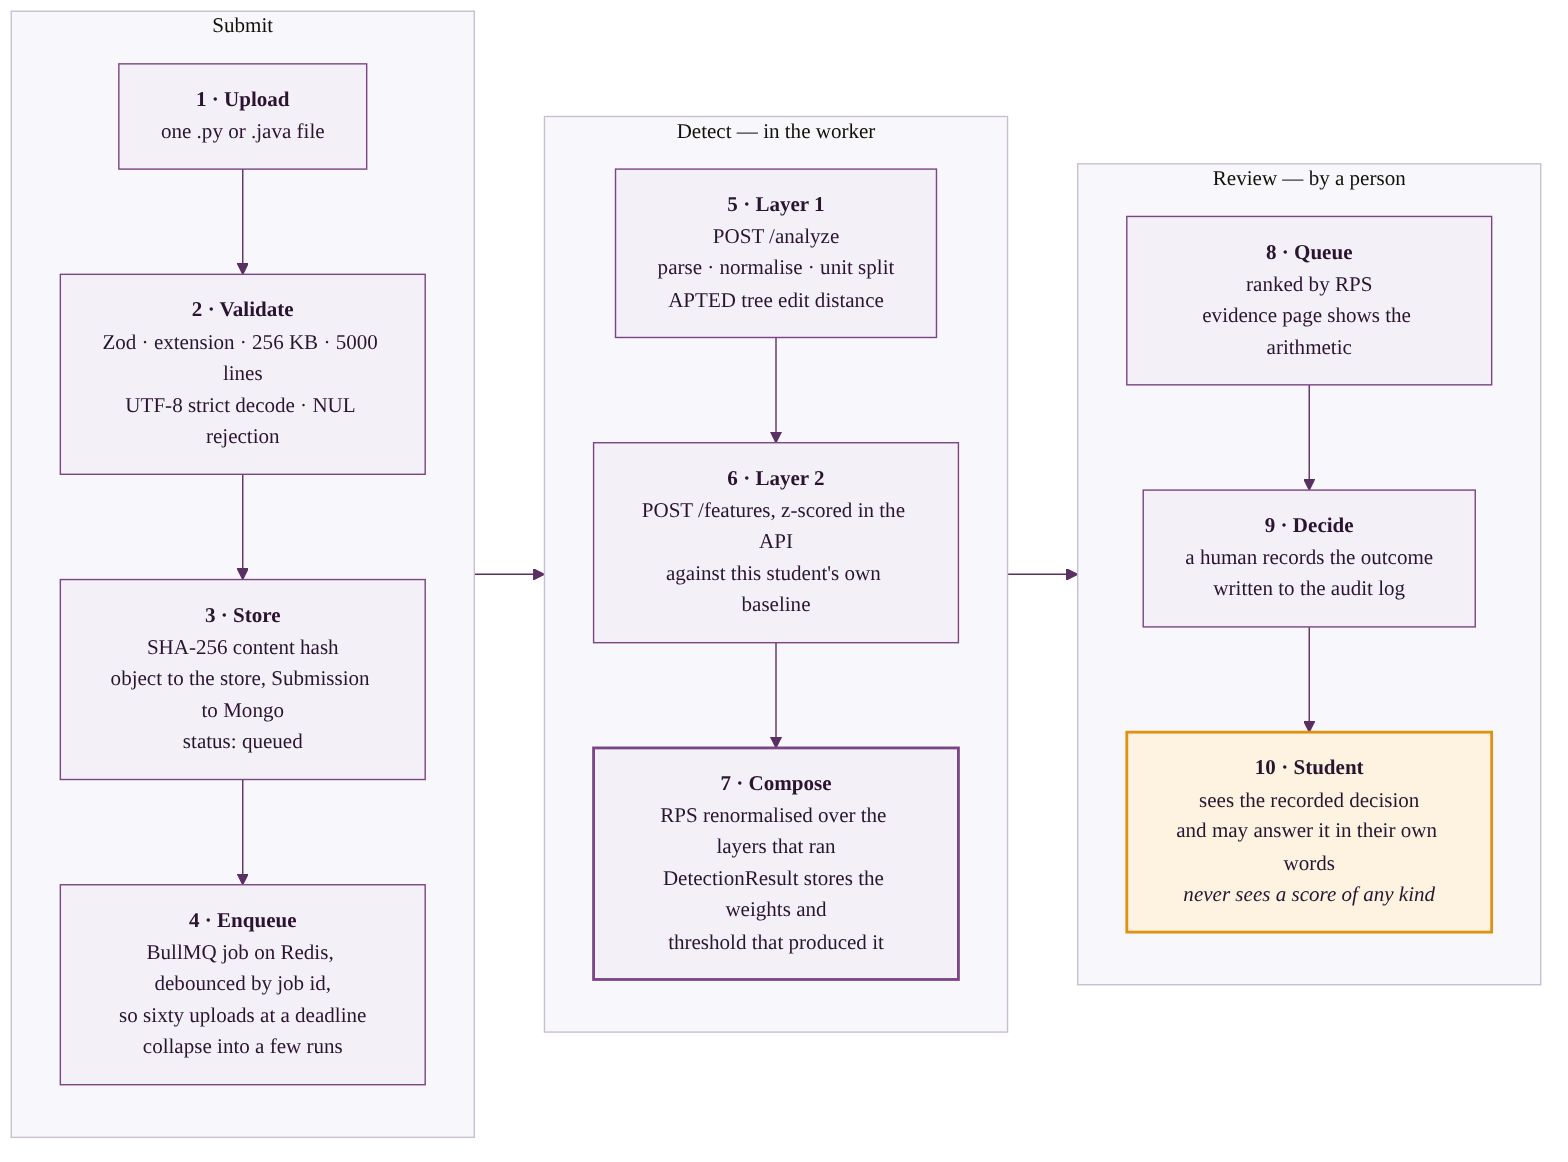
\includegraphics[width=\linewidth,height=0.78\textheight,keepaspectratio]{figures/02-data-flow.png}
\caption{One submission, end to end. Step 4 is debounced by job identity; step 7 stores the weights and threshold that produced the score; step 10 shows the student a decision and never a score.}
\label{fig:02-data-flow}
\end{figure}

Ten steps across three phases: upload, detection, review.

Three of the steps carry design decisions rather than mechanism.

\textbf{Step 4 is debounced by job identity.} Sixty uploads arriving at
a deadline collapse into a handful of detection runs rather than sixty,
because each run reads the current cohort anyway. Detection is slow ---
it parses, compares against candidates and waits on a second service ---
so performing it inside the upload request would make uploads take
seconds and fail under load at precisely the moment every student
submits at once.

\textbf{Step 7 stores the weights and the review threshold that produced
the score, on the result itself.} This is what lets the evidence page
stay readable after the configuration changes. Without it, a result
opened next term would be rendered against whatever weights happen to be
current, and its arithmetic would no longer add up.

\textbf{Step 10 is a design decision, not an omission.} The student sees
the recorded decision and may answer it, and never sees a score, because
a ranking a student can read is a ranking a student can tune against.

\hypertarget{data-model}{%
\section{Data model}\label{data-model}}

\begin{figure}[htbp]
\centering
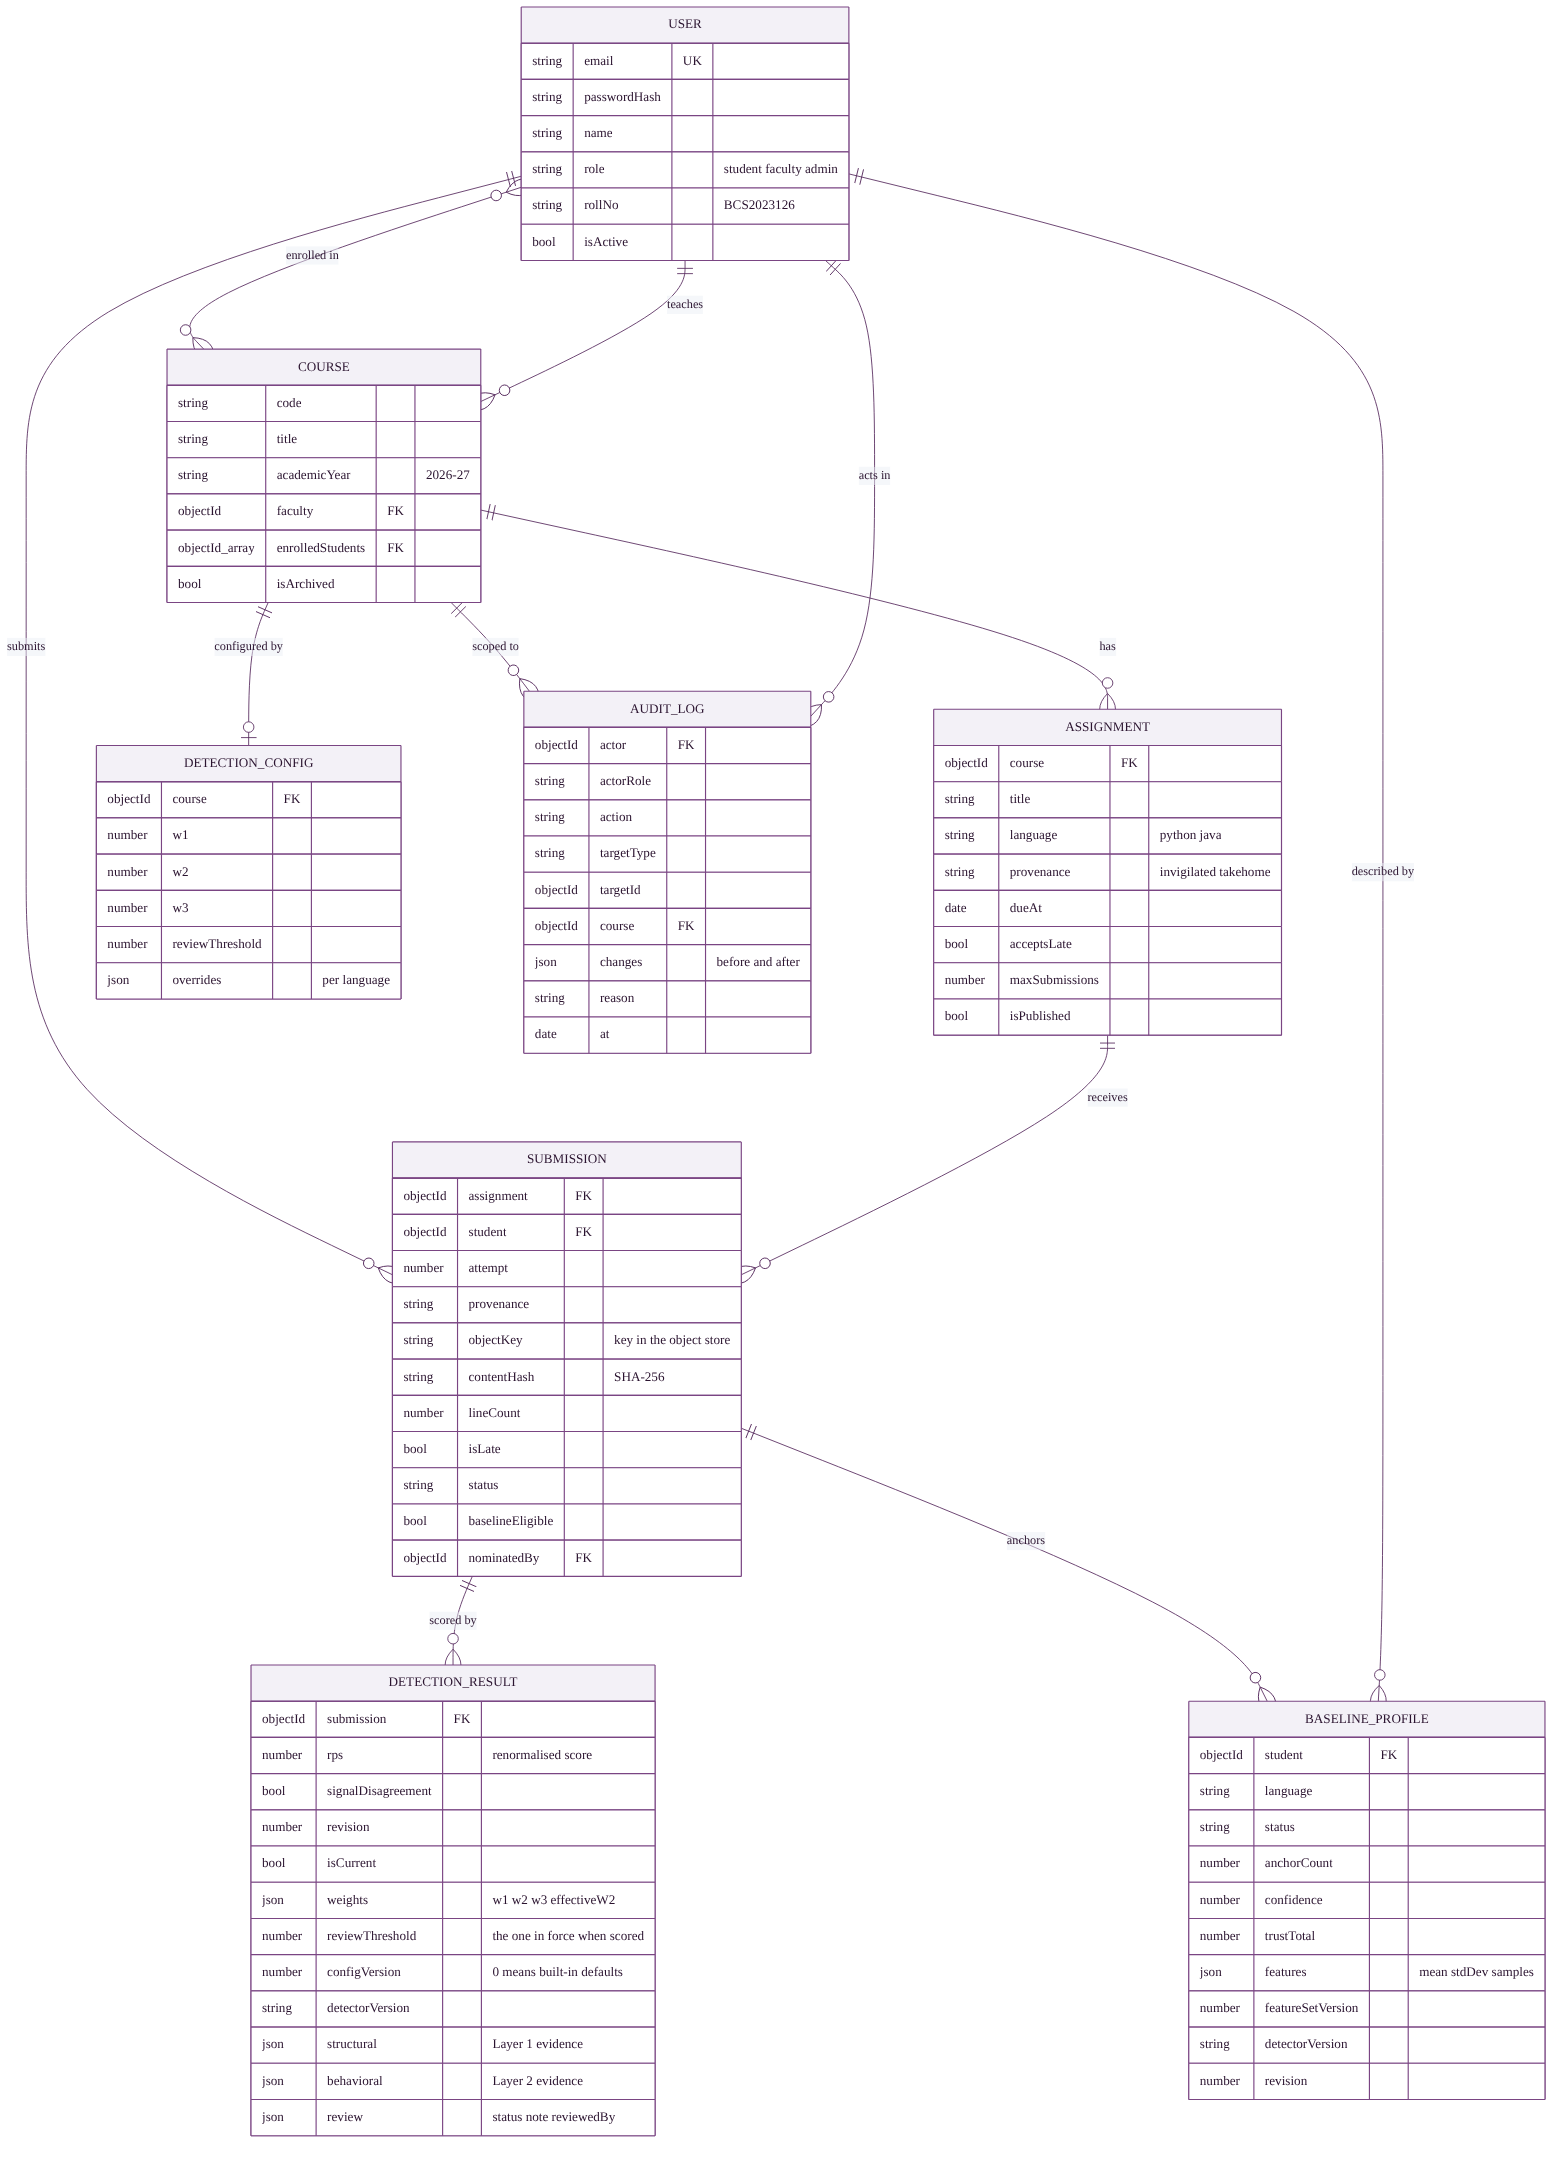
\includegraphics[width=\linewidth,height=0.78\textheight,keepaspectratio]{figures/03-data-model.png}
\caption{The eight collections. DetectionResult carries both layers' evidence rather than only their scores, and AuditLog is separate from the documents it describes.}
\label{fig:03-data-model}
\end{figure}

Eight collections: \texttt{User}, \texttt{Course}, \texttt{Assignment},
\texttt{Submission}, \texttt{DetectionResult}, \texttt{DetectionConfig},
\texttt{BaselineProfile} and \texttt{AuditLog}.

Three properties of the model are the ones to explain.

\textbf{\texttt{DetectionResult} carries both layers' evidence, not
merely their scores.} That is what makes the evidence page reproducible
from stored data rather than recomputed on demand. A score alone is an
assertion; the evidence beside it is what a reviewer can actually act on
and a student can contest.

\textbf{\texttt{isCurrent} and \texttt{revision} mean a re-run
supersedes a result without destroying it.} A decision may already have
been recorded against the earlier result, and destroying it would orphan
that decision.

\textbf{\texttt{AuditLog} is separate from the documents it describes},
so that the record of who changed what cannot be edited by the same
operation that changes the thing. An audit log a privileged operation
can rewrite is not an audit log.

\hypertarget{the-layer-2-pipeline}{%
\section{The Layer 2 pipeline}\label{the-layer-2-pipeline}}

\begin{figure}[htbp]
\centering
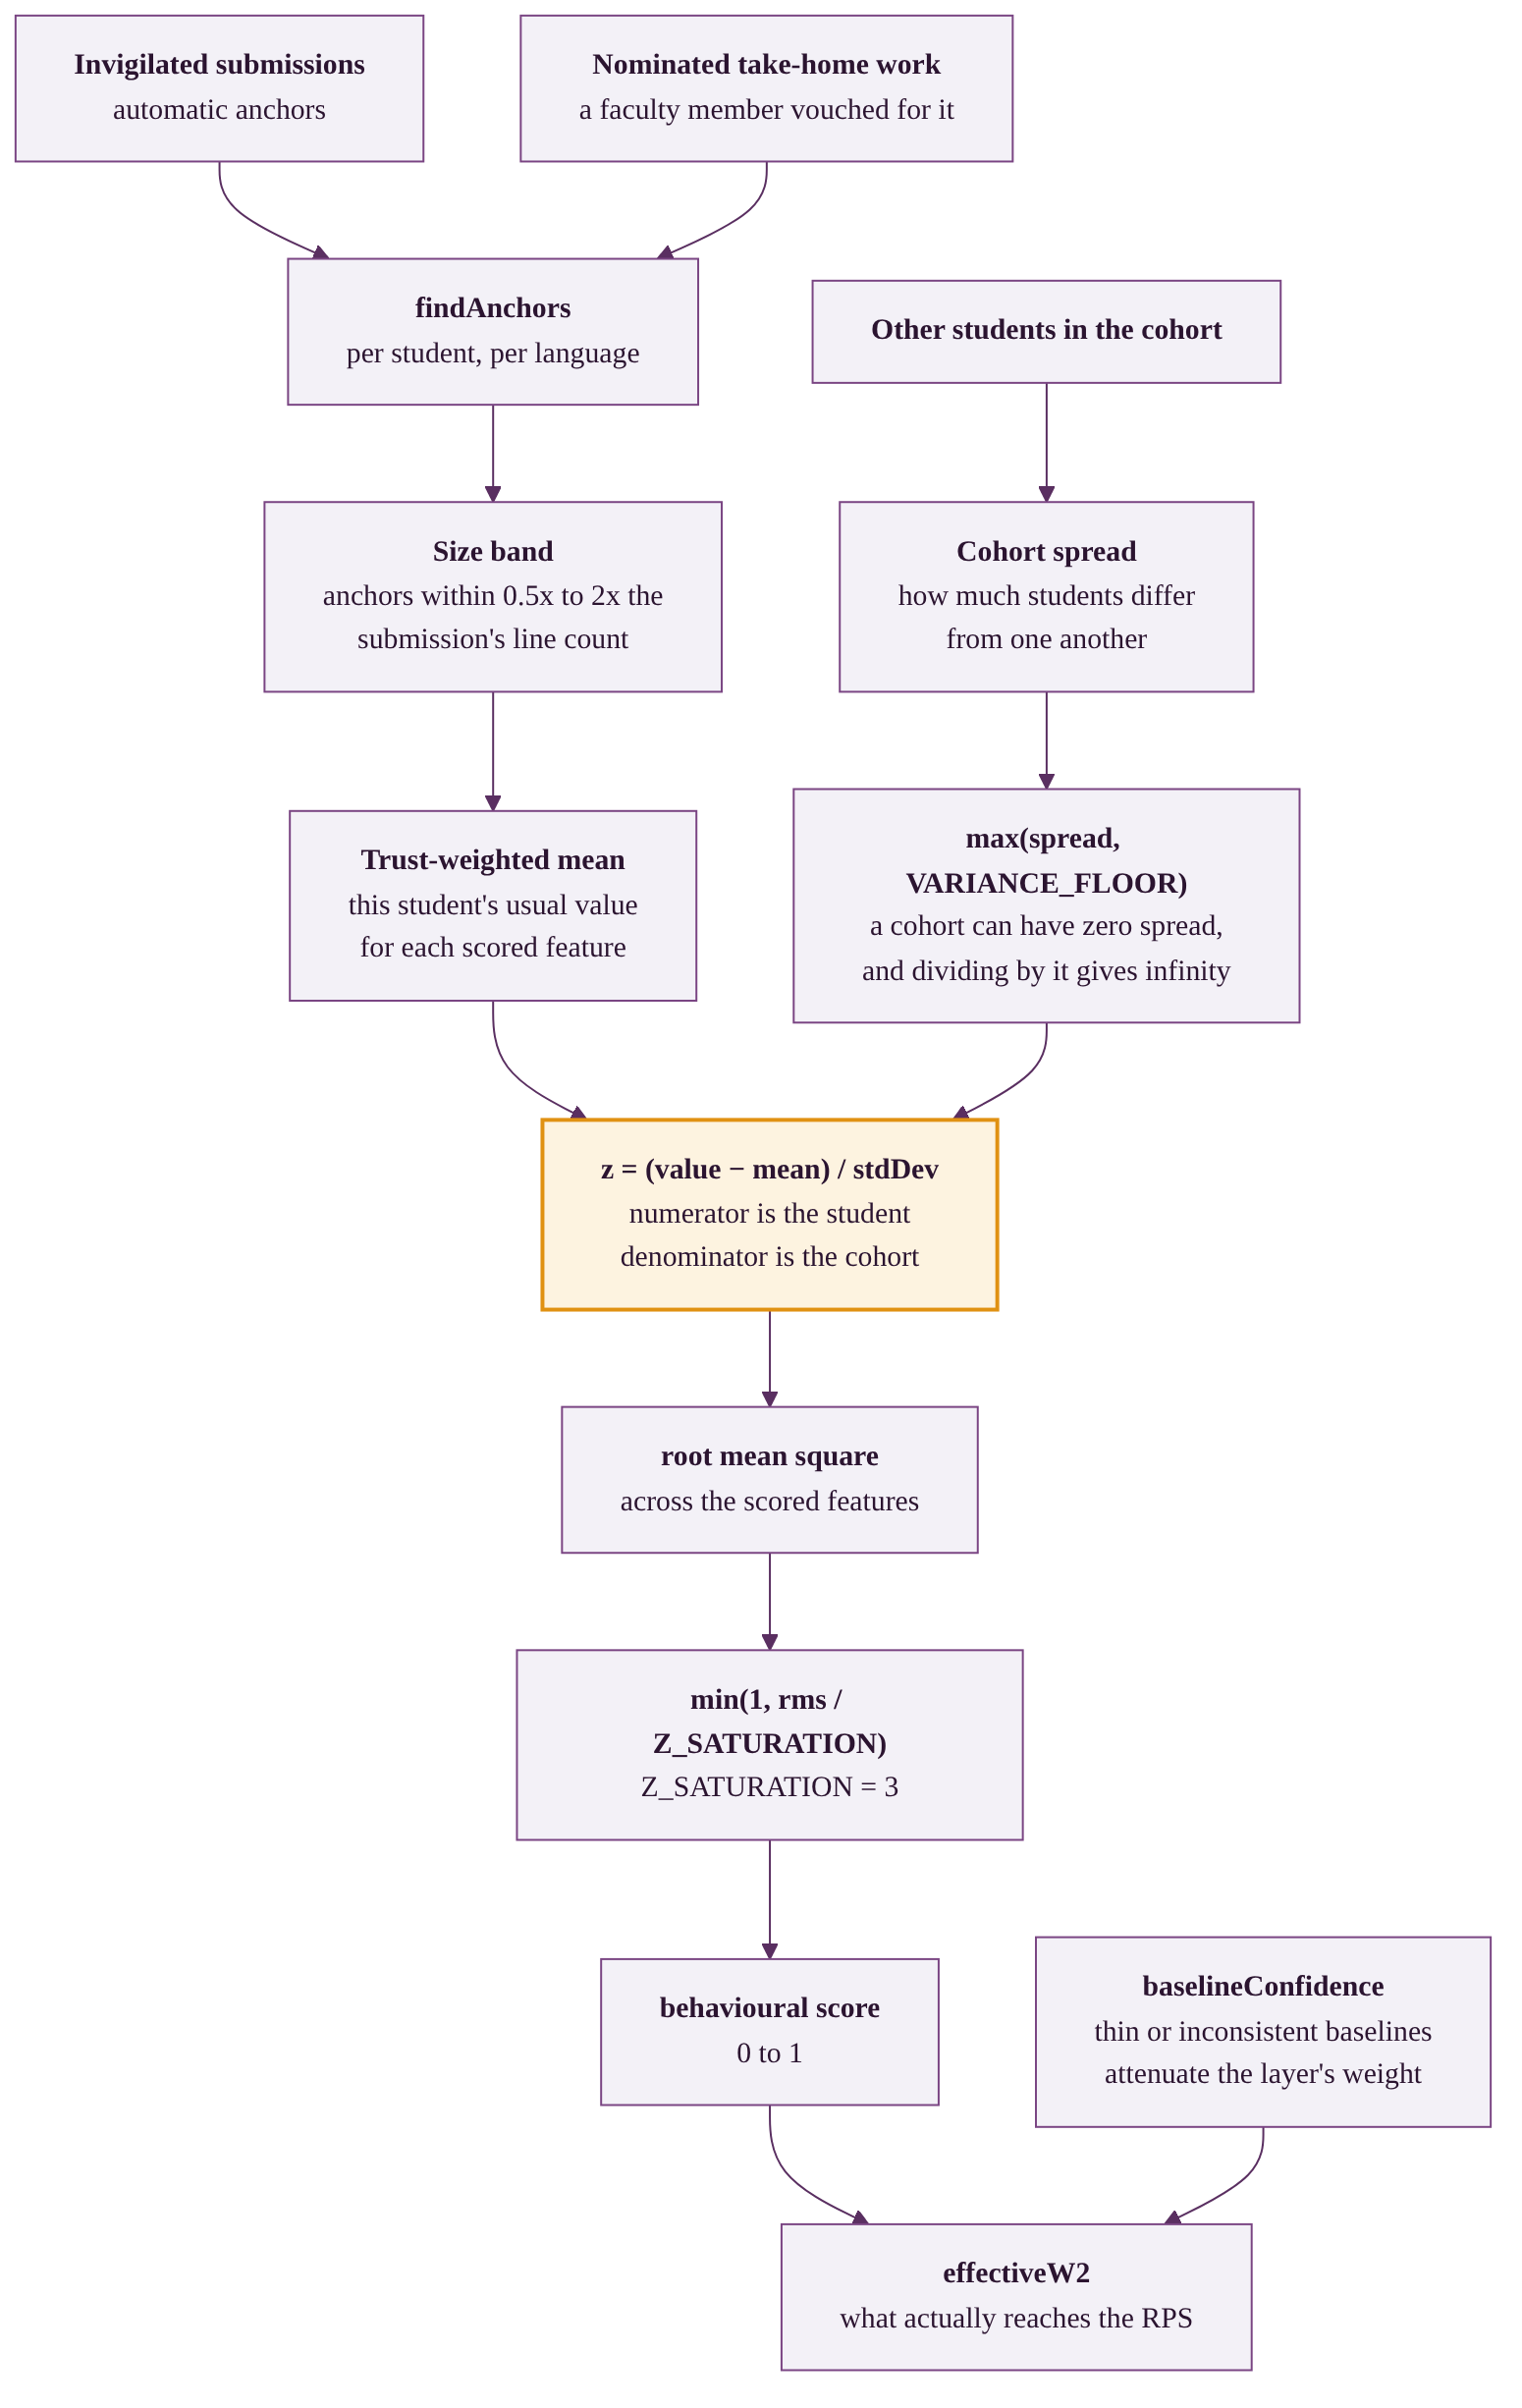
\includegraphics[width=\linewidth,height=0.78\textheight,keepaspectratio]{figures/04-layer2-pipeline.png}
\caption{The Layer 2 pipeline. The numerator comes from the student's own anchors, trust-weighted; the denominator comes from the cohort, floored.}
\label{fig:04-layer2-pipeline}
\end{figure}

This is the project's research contribution in one figure, and the first
place to look when defending it.

Note what joins at the z-score, because it is the thing most often
misread --- including in this project's own earlier documentation:

\begin{itemize}
\tightlist
\item
  the \textbf{numerator} comes from the student's own anchors,
  trust-weighted;
\item
  the \textbf{denominator} comes from the \textbf{cohort}, floored.
\end{itemize}

A z here means \emph{how far this submission sits from this student's
usual, measured in units of how much students in this class differ from
one another.} Both halves are load-bearing, and an earlier version of
the project documentation claimed the comparison was ``never against the
cohort'', which is false and would not survive an examiner opening the
file.

The floor exists because a cohort can produce zero spread on a coarse
feature, and dividing by zero gives infinity.

\textbf{The justification for the cohort denominator is an argument, not
a measurement, and the report must present it as such.} The argument is
that a student's own spread, estimated from three or four anchors, is
too unstable to divide by: a mean is personal, whereas a spread is
closer to a property of the feature. An AUC comparison previously quoted
in support of this has been retracted --- it is traceable to no run in
the measurements folder (Chapter 7 \S{}7.4) --- so the design choice stands
on its reasoning alone.

\hypertarget{composing-the-review-priority-score}{%
\section{Composing the Review Priority
Score}\label{composing-the-review-priority-score}}

\begin{figure}[htbp]
\centering
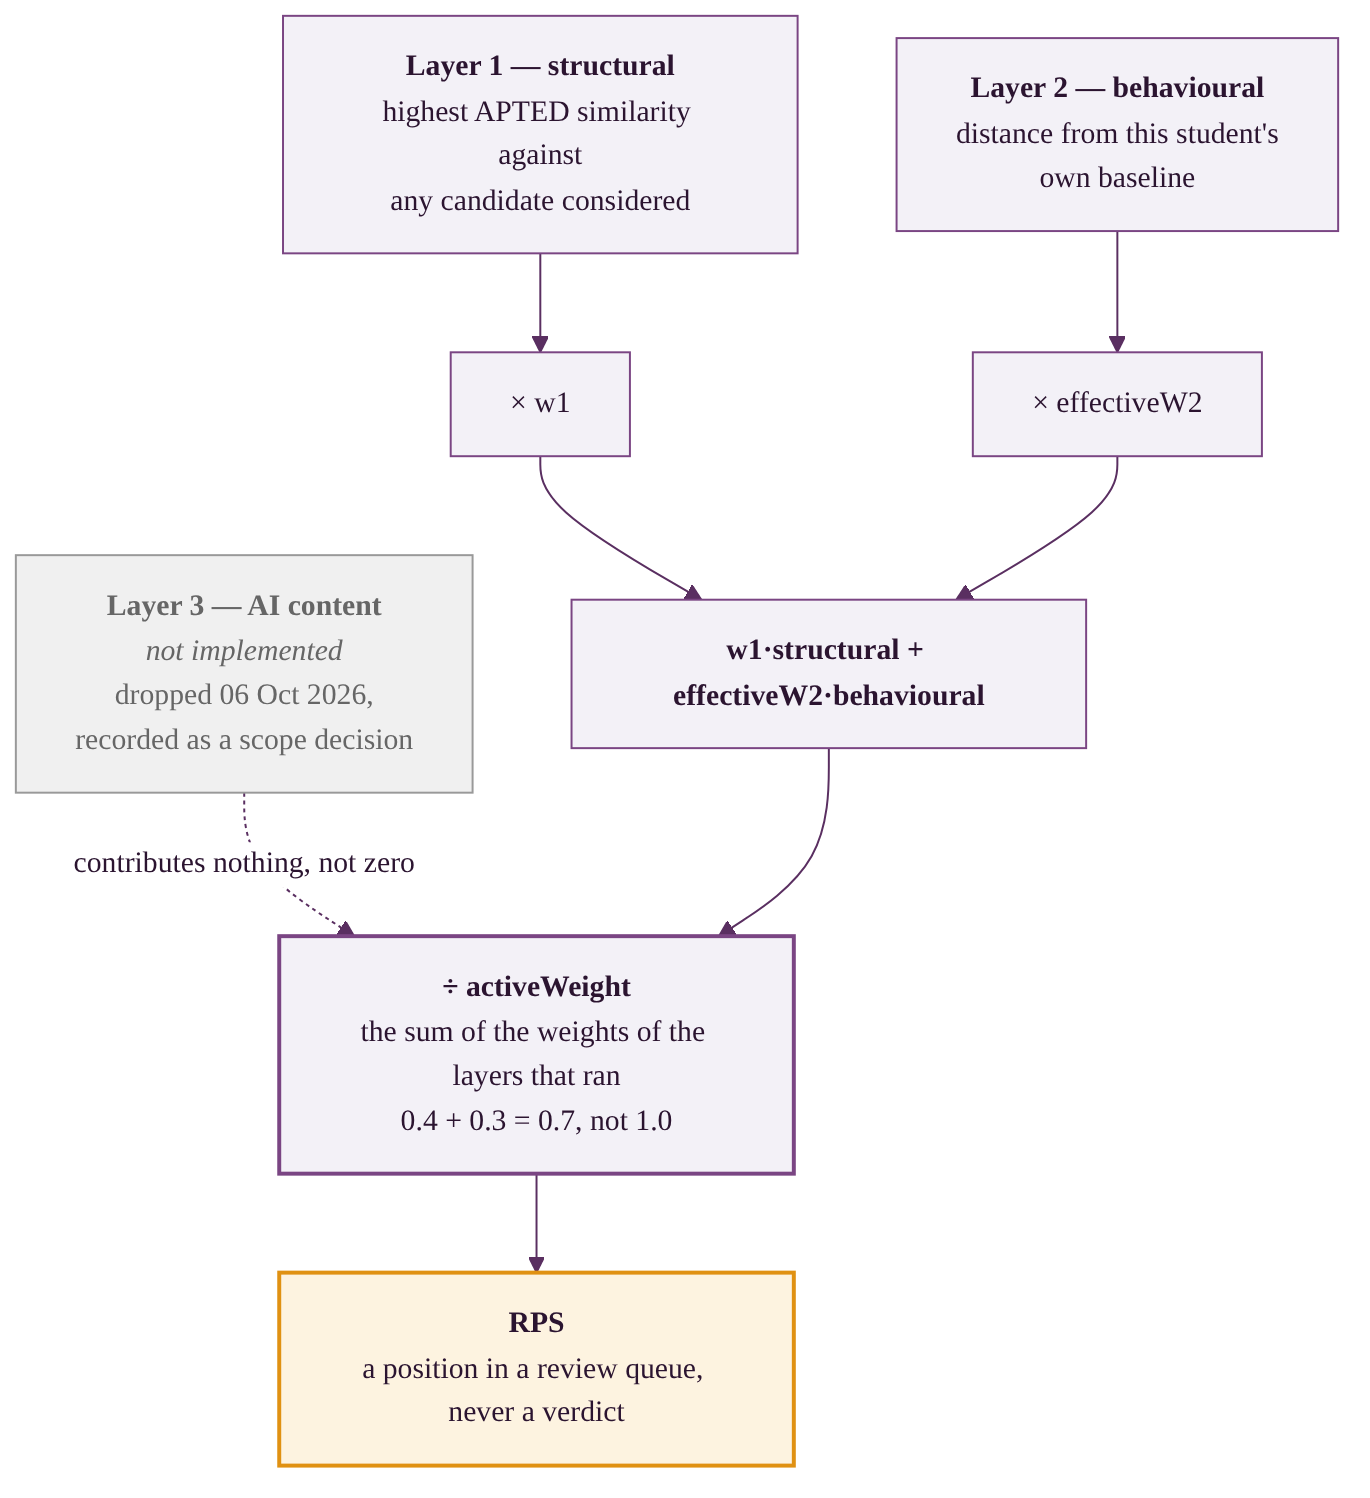
\includegraphics[width=\linewidth,height=0.78\textheight,keepaspectratio]{figures/05-rps-composition.png}
\caption{Composing the RPS. With Layer 3 absent the divisor is 0.7, so the configured 0.4/0.3/0.3 act as 0.571/0.429. An absent layer contributes nothing, not zero.}
\label{fig:05-rps-composition}
\end{figure}

\begin{verbatim}
activeWeight = (structuralOk ? w1 : 0) + (behaviouralOk ? effectiveW2 : 0)
RPS          = (w1 \textperiodcentered{} structural + effectiveW2 \textperiodcentered{} behavioural) / activeWeight
\end{verbatim}

\textbf{With Layer 3 absent, the configured weights 0.4 / 0.3 / 0.3 are
never the applied ones.} The divisor is the sum of the weights of the
layers that actually ran, which is 0.7, so they act as \textbf{0.571 /
0.429}. Quoting the configured triple as the operative weights would be
wrong, and the evidence page renders the renormalisation explicitly for
exactly this reason.

\textbf{An absent layer contributes nothing rather than contributing
zero}, because zero is a finding and an absent layer has made no
finding. Treating absence as zero would drag every score down by a third
and make a two-layer result incomparable with a three-layer one.

\texttt{effectiveW2} is Layer 2's weight after attenuation by baseline
confidence, so a thin baseline reduces the layer's influence instead of
being trusted at full strength. Figure 5 shows Layer 3 greyed and
excluded rather than omitted, because its absence is what makes the
renormalisation necessary.

\hypertarget{baseline-integrity-as-a-design-concern}{%
\section{Baseline integrity as a design
concern}\label{baseline-integrity-as-a-design-concern}}

Layer 2's failure mode is not a missed detection. It is a \textbf{wrong
baseline accusing an honest student}, and the design carries five
mitigations for it:

\begin{enumerate}
\def\labelenumi{\arabic{enumi}.}
\tightlist
\item
  \textbf{Anchor provenance} --- only invigilated work, or work a
  student nominates and faculty accept, may describe their style.
\item
  \textbf{Minimum anchor count} --- below three, the layer declines to
  score rather than guessing.
\item
  \textbf{Baseline confidence} --- a thin or inconsistent baseline
  attenuates the layer's weight instead of being trusted at full
  strength.
\item
  \textbf{Low-variance flag} --- a student whose own work varies less
  than the cohort's is penalised by z-scoring, and the result says so.
\item
  \textbf{Cohort saturation flag} --- when the pooled spread collapses,
  every z-score is a real difference divided by an invented floor, and
  the layer has stopped discriminating. The result says that too.
\end{enumerate}

Mitigations 2 to 5 share a character worth naming in the report:
\textbf{the system reports that it cannot tell, rather than producing a
number that looks like an answer.} That is what an evidence system owes
a reviewer, and it is the design-level expression of the principle in
Chapter 2 \S{}2.2 that a tool does not determine plagiarism.

\hypertarget{what-the-diagrams-deliberately-do-not-show}{%
\section{What the diagrams deliberately do not
show}\label{what-the-diagrams-deliberately-do-not-show}}

These figures show the system that exists, not the system the project
presentation describes. Three items in that deck are absent here because
they are absent in the code, and the report carries them as scope
decisions rather than letting an examiner find the gap:

\begin{itemize}
\tightlist
\item
  \textbf{Layer 3, CodeBERT.} Dropped 06 October 2026. Figure 5 shows it
  greyed and excluded rather than omitting it, because its absence is
  what makes the renormalisation necessary. The reasoning is in Chapter
  5 \S{}5.4.
\item
  \textbf{The WebSocket push.} Not built. The queue is polled by the
  reviewer rather than pushed to them.
\item
  \textbf{The side-by-side AST diff.} Not built. The evidence page shows
  matching line ranges and links to each file; rendering the two sources
  against each other needs a diff view that was not implemented.
\end{itemize}

\hypertarget{implementation-how-the-system-works}{%
\chapter{Implementation: how the system
works}\label{implementation-how-the-system-works}}

\begin{draftnote}

\textbf{Draft status, 03 November 2026.} Written from the implemented
code and from \texttt{docs/PROJECT\_STATUS.md}. Every constant quoted
below is named in the source; \textbf{check each against the file cited
beside it before submission}, because a constant quoted wrongly in a
report is the easiest thing for an examiner to catch and the hardest to
recover from. Figures 1 to 5 referred to here are the committed diagrams
in \texttt{docs/diagrams/}.

\end{draftnote}

\begin{center}\rule{0.5\linewidth}{0.5pt}\end{center}

\hypertarget{the-stack-and-why-each-part-is-where-it-is}{%
\section{The stack, and why each part is where it
is}\label{the-stack-and-why-each-part-is-where-it-is}}

\begin{longtable}[]{@{}
  >{\raggedright\arraybackslash}p{(\columnwidth - 4\tabcolsep) * \real{0.3333}}
  >{\raggedright\arraybackslash}p{(\columnwidth - 4\tabcolsep) * \real{0.3333}}
  >{\raggedright\arraybackslash}p{(\columnwidth - 4\tabcolsep) * \real{0.3333}}@{}}
\toprule\noalign{}
\begin{minipage}[b]{\linewidth}\raggedright
tier
\end{minipage} & \begin{minipage}[b]{\linewidth}\raggedright
technology
\end{minipage} & \begin{minipage}[b]{\linewidth}\raggedright
reason
\end{minipage} \\
\midrule\noalign{}
\endhead
\bottomrule\noalign{}
\endlastfoot
Web client & React 19, Vite & the examiner-facing demonstration; holds
no credentials \\
API & Node, Express 5, TypeScript, Mongoose & the only tier that holds
credentials or reaches a store \\
Detector & Python, FastAPI, tree-sitter, APTED & the parsing and tree
libraries that exist are Python ones \\
Documents & MongoDB & the detection result is a nested document, not a
set of rows \\
Queue & Redis & detection is slow and must not block an upload \\
Files & MinIO-compatible object store & submitted source is a blob, not
a column \\
\end{longtable}

The split between API and detector is the one design decision worth
defending in a viva, because it looks like unnecessary complexity for a
student project. It is not. The parsing ecosystem this project needs ---
tree-sitter grammars and an APTED implementation --- is Python. The web
application and its data model are far more naturally expressed in
TypeScript against Mongoose. Rather than compromise one to accommodate
the other, the system makes the detector a stateless HTTP service that
parses and compares, and keeps every piece of state, every credential
and every authorisation decision in the API.

The worker is deliberately \emph{not} a separate codebase. It is the API
started on a different entry point, so a queued detection job and a
synchronous request share one set of services. Two implementations of
the same scoring logic would drift, and the drift would appear as a
result that cannot be reproduced.

\hypertarget{layer-1-structural-similarity-in-working-order}{%
\section{Layer 1 --- structural similarity, in working
order}\label{layer-1-structural-similarity-in-working-order}}

Layer 1 answers \emph{does this submission resemble another submission?}
Its chain runs through four stages, and the stages matter because two of
them operate on different representations of the same file.

\hypertarget{parsing}{%
\subsection{Parsing}\label{parsing}}

\texttt{app/parsing.py} exposes
\texttt{parse\_source(language,\ source)}, returning a
\texttt{ParseResult} carrying \texttt{ok}, \texttt{node\_count},
\texttt{error} and \texttt{root}. One detail is load-bearing and caused
a real defect during the measurement work: \textbf{the root is returned
even when the parse fails.} tree-sitter \cite{treesitter} is an
error-recovering parser, so a syntactically broken file still yields a
tree. Any caller that tests \texttt{root\ is\ None} rather than
\texttt{ok} will therefore proceed on a tree built from broken source.
Callers test \texttt{ok}.

\hypertarget{normalisation}{%
\subsection{Normalisation}\label{normalisation}}

\texttt{app/normalise.py} turns the raw tree-sitter tree into a
\texttt{TNode} tree via \texttt{normalise(node)}. Normalisation is where
the resistance to obfuscation comes from: identifier names, literal
values and formatting are discarded, and each node carries a
\texttt{label} describing its syntactic kind rather than its text. This
is what makes renaming a variable invisible to Layer 1.

\textbf{The two representations are not interchangeable, and the report
should say so plainly}, because it is the clearest illustration of what
each layer is looking at:

\begin{itemize}
\tightlist
\item
  Layer 1 consumes the \textbf{normalised} tree, because structure is
  what survives obfuscation.
\item
  Layer 2 consumes the \textbf{raw} tree, because style lives precisely
  in the things normalisation throws away --- blank lines, comments,
  line lengths.
\end{itemize}

The same source file is therefore read twice, in two different ways, for
two different questions. \texttt{extract\_units} and \texttt{size} take
the normalised tree; \texttt{extract\_features} takes the raw root and
the source bytes.

\hypertarget{unit-extraction}{%
\subsection{Unit extraction}\label{unit-extraction}}

\texttt{app/units.py} provides \texttt{extract\_units(tree,\ language)},
which splits a normalised tree into comparable top-level units ---
functions, methods, classes --- rather than treating the file as one
monolithic tree. Comparing whole files would make a long honest file
resemble another long honest file simply by virtue of both being long.
Comparing unit against unit allows the system to report \emph{which}
parts matched, which is what a reviewer needs.

\hypertarget{prefilter-the-step-that-makes-it-affordable}{%
\subsection{Prefilter: the step that makes it
affordable}\label{prefilter-the-step-that-makes-it-affordable}}

\texttt{app/prefilter.py} exists because tree edit distance is
expensive. It builds a \texttt{Counter} of node labels per tree ---
\texttt{label\_counts} --- and scores candidate pairs by bag overlap
with \texttt{quick\_similarity}, which is cheap and approximate and
never final. \texttt{rank} then nominates the most promising candidates.

Two constants from \texttt{app/main.py} govern the cost:

\begin{itemize}
\tightlist
\item
  \texttt{MAX\_CANDIDATES\ =\ 50} --- the most candidates the endpoint
  will accept at all.
\item
  \texttt{MAX\_DEEP\_CANDIDATES\ =\ 10} --- of those, how many earn the
  expensive treatment.
\end{itemize}

So a submission is compared in full against at most ten candidates
however large the cohort is. This bounds one analysis irrespective of
class size, and it is also a \textbf{fidelity requirement on any
measurement of Layer 1}: a study that compares exhaustively is measuring
a system that was never deployed, and will credit the layer with matches
the API cannot find. That error was made and corrected during this
project's own ablation work, and Chapter 7 records it.

\texttt{shortlist\_pairs} nominates pairs from \emph{both} directions.
Shortlisting in one direction starves units nobody happens to pick: if
every unit of A nominates the same five units of B, the remainder of B
is never offered to anyone and their partners in A go unmatched.

\hypertarget{comparison-and-scoring}{%
\subsection{Comparison and scoring}\label{comparison-and-scoring}}

\texttt{compare\_unit\_sets(units\_a,\ units\_b,\ size\_a,\ size\_b)}
returns a \texttt{FileComparison} carrying the similarity, the matched
unit pairs, coverage on each side, and counts of pairs compared, pruned
and skipped. The underlying distance is APTED \cite{pawlik2016}, with
RTED \cite{pawlik2015} as the algorithmic predecessor the authors ask to
be cited alongside.

Reported evidence is filtered: \texttt{MIN\_SPAN\_NODES\ =\ 10}
suppresses matches too small to mean anything, because two one-line
functions resemble each other by virtue of being one line long. The
filter applies to the \emph{spans shown to a reviewer}, not to the
similarity figure itself --- a distinction worth knowing before
answering a question about it.

\hypertarget{layer-2-behavioural-fingerprinting-in-working-order}{%
\section{Layer 2 --- behavioural fingerprinting, in working
order}\label{layer-2-behavioural-fingerprinting-in-working-order}}

Layer 2 answers a different question: \emph{does this submission
resemble its own author's previous work?} It is the only layer that can
see outsourced work, because it needs no second copy anywhere.

\hypertarget{features}{%
\subsection{Features}\label{features}}

The detector's \texttt{/features} endpoint extracts \textbf{ten}
features via \texttt{app/features.py}: \texttt{avg\_line\_length},
\texttt{blank\_line\_ratio}, \texttt{comment\_density},
\texttt{avg\_identifier\_length},
\texttt{underscore\_identifier\_ratio}, \texttt{avg\_function\_lines},
\texttt{functions\_per\_100\_lines}, \texttt{max\_block\_depth},
\texttt{avg\_params\_per\_function} and \texttt{for\_loop\_ratio}. All
ten are stored on the baseline.

\textbf{Four are scored.} \texttt{SCORED\_FEATURES} in
\texttt{services/behavioural.ts} is \texttt{blank\_line\_ratio},
\texttt{avg\_line\_length}, \texttt{max\_block\_depth},
\texttt{comment\_density}. Storing all ten keeps the choice reversible.

The justification for choosing those four is \textbf{retracted}, and the
report must say so rather than repeat it. The four were selected from a
60-file sample; a later measurement over 204 Python files across 15
repositories found that the earlier ranking does not replicate, that
\texttt{blank\_line\_ratio} --- which had driven the choice --- ranks
ninth of ten in Python, and that using every applicable feature beats
the fixed four in both languages. Chapter 7 carries the figures.

\hypertarget{anchors-and-the-baseline}{%
\subsection{Anchors and the baseline}\label{anchors-and-the-baseline}}

\texttt{services/anchors.ts} decides which past submissions may describe
a student's style, and \texttt{services/baseline.ts} builds the
per-student, per-language profile from them. Eligibility is the first of
the five integrity mitigations below.

\hypertarget{the-score-and-what-its-two-halves-mean}{%
\subsection{The score, and what its two halves
mean}\label{the-score-and-what-its-two-halves-mean}}

\begin{verbatim}
z        = (value - mean) / stdDev
stdDev   = max(cohortSpread, VARIANCE_FLOOR[feature])
score    = min(1, rootMeanSquare(z) / Z_SATURATION)      Z_SATURATION = 3
\end{verbatim}

The asymmetry here is the project's central idea and the thing most
likely to be misread, including in its own earlier documentation:

\begin{itemize}
\tightlist
\item
  the \textbf{numerator} is the student's own trust-weighted mean across
  their anchors;
\item
  the \textbf{denominator} is the \textbf{cohort's} spread, floored.
\end{itemize}

A z-score therefore means \emph{how far this submission sits from this
student's usual, measured in units of how much students in this class
differ from one another}. Both halves are load-bearing. An earlier
version of this project's documentation claimed the comparison was
``never against the cohort'', which is false and does not survive an
examiner opening the file.

The cohort denominator is a measured choice rather than a convenience: a
student's own spread, taken from three or four anchors, is too unstable
to divide by. A student's mean is personal; the spread is closer to a
property of the feature. The variance floor exists because a cohort can
produce zero spread on a coarse feature, and dividing by zero gives
infinity.

\textbf{The AUC figures previously quoted here are retracted} --- 0.766
for a student's own spread against 0.909 for the cohort's. No
measurement script computes an AUC; see Chapter 7 \S{}7.4. The cohort
denominator rests on the stability argument above, which is reasoning
rather than measurement.

\hypertarget{the-five-baseline-integrity-mitigations}{%
\subsection{The five baseline-integrity
mitigations}\label{the-five-baseline-integrity-mitigations}}

Layer 2's failure mode is not a false negative; it is a wrong baseline
accusing an honest student. Five mitigations exist, and they are a
genuine contribution of the project rather than boilerplate:

\begin{enumerate}
\def\labelenumi{\arabic{enumi}.}
\tightlist
\item
  \textbf{Anchor provenance.} Only invigilated work, or work a student
  nominates and faculty accept, may describe their style.
\item
  \textbf{Minimum anchor count.} Below \texttt{minAnchorsForBaseline}
  (3) the layer declines to score rather than guessing.
\item
  \textbf{Baseline confidence.} A thin or inconsistent baseline
  attenuates the layer's weight (\texttt{effectiveW2}) instead of being
  trusted at full strength.
\item
  \textbf{Low-variance flag.} A student whose own work varies less than
  the cohort's is penalised by z-scoring, and the result says so.
\item
  \textbf{Cohort saturation flag.} When the pooled spread collapses,
  every z-score is a real difference divided by an invented floor, and
  the layer has stopped discriminating. The result says that too.
\end{enumerate}

Mitigations 2, 3, 4 and 5 all have the same character: the system
reports that it cannot tell, instead of producing a number that looks
like an answer. That is the behaviour an evidence system owes a
reviewer.

\hypertarget{layer-3-specified-justified-and-not-built}{%
\section{Layer 3 --- specified, justified, and not
built}\label{layer-3-specified-justified-and-not-built}}

\textbf{Layer 3 is not implemented.} This section states the decision
and its reasoning, because an unexplained hole where a third of the
architecture should be is worse than a documented exclusion.

The layer would have detected machine-generated code, following the
CodeBERT fine-tuning approach of Nguyen et
al.~\cite{nguyen2023, gptsniffer2024}. That work reports two findings
that together make the layer unbuildable \emph{as evidence} in this
setting: classifier performance improves when the training data
resembles the target code, and when snippets are classified in pairs.

A classifier whose accuracy depends on in-distribution training data
requires a labelled corpus of student submissions from the course it
will police. No such corpus exists for this project, and one cannot be
manufactured honestly --- generating synthetic ``AI-written''
submissions and treating them as ground truth would produce a figure
that measures the generator, not the classifier.

The layer could still have been \emph{implemented}. What it could not be
is \emph{characterised}. In a system whose entire premise is auditable
evidence, a layer that emits a number nobody can put a confidence
interval on is worse than an absent layer, because a reviewer has no
basis on which to weigh it against the layers that are measured.

The decision is recorded in the data rather than in a comment. Every
detection result stores:

\begin{verbatim}
aiContent: { status: "skipped", reason: "Layer 3 is not implemented yet" }
\end{verbatim}

so that a result read years later says why it has two layers and not
three. Chapter 8 lists the layer as future work with the labelled corpus
named as its precondition.

\hypertarget{composing-the-review-priority-score}{%
\section{Composing the Review Priority
Score}\label{composing-the-review-priority-score}}

\begin{verbatim}
activeWeight = (structuralOk ? w1 : 0) + (behaviouralOk ? effectiveW2 : 0)
RPS          = (w1 * structural + effectiveW2 * behavioural) / activeWeight
\end{verbatim}

\texttt{services/detection.ts} performs this composition. Three
properties of it are worth a paragraph each in the report, and Figure 5
illustrates them.

\textbf{The configured weights are never the applied ones.} The
configuration carries 0.4 / 0.3 / 0.3 across three layers. With Layer 3
absent the divisor is the sum of the weights of the layers that ran,
which is 0.7, so the applied weights are \textbf{0.571 and 0.429}.
Quoting 0.4 / 0.3 / 0.3 as the operative weights would be wrong, and the
evidence page renders the renormalisation explicitly for this reason.

\textbf{An absent layer contributes nothing, not zero.} The distinction
is not pedantry. A zero is a finding --- it asserts that the layer
looked and found nothing. An absent layer has not looked. Treating
absence as zero would drag every score down by a third and make a
two-layer result incomparable with a three-layer one.

\textbf{The weights and threshold are stored on the result.}
\texttt{effectiveW2} is Layer 2's weight after attenuation by baseline
confidence, and both it and the review threshold are written onto each
\texttt{DetectionResult}. A result therefore remains readable after the
configuration changes, which is what makes the evidence view
reproducible from stored data instead of recomputed against whatever the
configuration happens to be when someone opens it.

\hypertarget{the-queue-and-why-detection-is-not-synchronous}{%
\section{The queue, and why detection is not
synchronous}\label{the-queue-and-why-detection-is-not-synchronous}}

Detection is slow: it parses, it compares against candidates, and it
waits on a second service. Doing it inside the upload request would make
an upload take seconds and fail under load at precisely the moment every
student submits.

\texttt{POST\ /submissions} therefore stores the file, records the
submission and enqueues the work on Redis, \textbf{debounced by job
identity} (Figure 2, step 4). Sixty uploads arriving at a deadline
collapse into a bounded number of detection runs rather than sixty,
because each run reads the current cohort anyway.

A re-run supersedes rather than replaces: \texttt{DetectionResult}
carries \texttt{isCurrent} and \texttt{revision}, so the superseded
result survives. A decision may already have been recorded against it,
and destroying the result would orphan the decision.

\hypertarget{the-web-interface}{%
\section{The web interface}\label{the-web-interface}}

Ten pages and five shared components in \texttt{apps/web}, built between
14 and 26 October. The three worth discussing in the report are:

\begin{itemize}
\tightlist
\item
  \textbf{The review queue} --- assignments ranked by RPS descending,
  showing each student's name and roll number. The roll number is not
  decoration: a fixture containing two students sharing a surname made
  it necessary.
\item
  \textbf{The evidence page} --- the system's actual thesis made
  visible. It renders the caveats \emph{before} the number, the
  per-feature breakdown, the matched spans, and the renormalisation
  arithmetic. It also \textbf{guards its own equation}: it recomputes
  the RPS from the stored weights and, where the recomputation and the
  stored score disagree by more than a small tolerance, refuses to
  render the equation and says the two disagree, rather than printing an
  identity that does not hold.
\item
  \textbf{The student's own result view} --- status, any recorded
  decision, and a form to answer it. \textbf{No score appears anywhere
  on it}, because the endpoint it reads returns none. A ranking a
  student can read is a ranking a student can tune against.
\end{itemize}

A methodology note belongs in Chapter 6 rather than here, but it
originates in this work: rendering real data through these screens found
defects the test suite had not, and printing them to paper found more. A
test asserts a value; these were things nobody had thought to assert.

\hypertarget{what-is-deliberately-not-built}{%
\section{What is deliberately not
built}\label{what-is-deliberately-not-built}}

Stated here so that the presentation's architecture slides and the
delivered system can be reconciled rather than silently differing:

\begin{itemize}
\tightlist
\item
  \textbf{Layer 3}, for the reasons in \S{}5.4.
\item
  \textbf{WebSocket push} for queue updates. The queue is polled by the
  reviewer.
\item
  \textbf{Side-by-side AST diff} rendering of two sources. The evidence
  page reports matching line ranges and links to each file; rendering
  both sources against each other needs a diff view that was not built.
\item
  \textbf{Multi-file and archive submissions.} One source file per
  submission.
\end{itemize}

\hypertarget{testing-and-verification}{%
\chapter{Testing and Verification}\label{testing-and-verification}}

\begin{draftnote}

\textbf{Draft status, 04 November 2026.} Figures read from
\texttt{docs/TESTING.md}, \texttt{apps/api/package.json},
\texttt{apps/api/tests/helpers.ts}, \texttt{.github/workflows/ci.yml}
and \texttt{docs/PROJECT\_NOTES.md}. Re-run the suite and confirm the
counts before submission; a test count quoted wrongly is the easiest
thing for an examiner to check.

\end{draftnote}

\begin{center}\rule{0.5\linewidth}{0.5pt}\end{center}

\hypertarget{what-is-tested-and-what-that-number-means}{%
\section{What is tested, and what that number
means}\label{what-is-tested-and-what-that-number-means}}

\textbf{278 automated tests: 155 in the API under vitest, 123 in the
detector under pytest.}

The split is not arbitrary. The detector suite covers the whole
structural tier --- parsing, normalisation, tree edit distance, the
prefilter, unit matching, the style-feature extraction and both HTTP
endpoints --- and needs no database, no object store and no Docker. It
runs in under three seconds and is the fastest useful signal in the
project. The API suite covers authentication, courses, submissions,
results, the configuration resolver, Layer 2 and the re-run path, and
needs MongoDB, Redis and the object store running.

A count on its own is close to meaningless, so the rest of this chapter
is about what the suite is constructed to prevent rather than how much
of it there is.

\hypertarget{three-design-decisions-in-the-test-harness}{%
\section{Three design decisions in the test
harness}\label{three-design-decisions-in-the-test-harness}}

These are worth a chapter section because each one exists in response to
a specific way the suite could have produced false results.

\hypertarget{a-guard-that-refuses-to-run-against-the-development-database}{%
\subsection{A guard that refuses to run against the development
database}\label{a-guard-that-refuses-to-run-against-the-development-database}}

\texttt{tests/helpers.ts} rewrites the Mongo URI to point at
\texttt{codeguard\_test}, and then refuses to proceed if the rewrite did
not take effect:

\begin{verbatim}
process.env.MONGO_URI = (process.env.MONGO_URI ?? "").replace("/codeguard?", `/${TEST_DB}?`);
if (!process.env.MONGO_URI.includes(`/${TEST_DB}?`)) {
  throw new Error(`Refusing to run: tests must use the ${TEST_DB} database`);
}
\end{verbatim}

The suite clears collections between tests. Without this guard, a
mistyped or unset URI would point that clearing at the development
database. The guard is the thing standing between a typo and the loss of
every fixture, course and submission in local development.

It has a consequence worth knowing: the \texttt{.env} path is
\textbf{relative to the working directory}, so running the suite from
the repository root loads nothing, leaves \texttt{MONGO\_URI} empty, and
produces 155 identical failures on that error message. \textbf{That is
the guard working, not 155 real failures} --- a distinction that costs a
quarter of an hour the first time it happens.

\hypertarget{serial-execution-because-the-files-share-one-database}{%
\subsection{Serial execution, because the files share one
database}\label{serial-execution-because-the-files-share-one-database}}

\begin{verbatim}
"test": "vitest run --no-file-parallelism"
\end{verbatim}

Every test file connects to the same database and clears collections
between tests. Run the files in parallel and they delete each other's
fixtures mid-run. The failures that produces are real-looking, entirely
fictional, and move around between runs --- the worst category of red to
debug, because it punishes the correct instinct of re-running to
confirm.

\texttt{npm\ test} also runs \texttt{pretest}, which typechecks first,
so a drifted contract is caught in seconds before any container is
touched. Calling \texttt{vitest} directly loses both properties, which
is why the project's documentation specifies \texttt{npm\ test} rather
than the tool underneath it.

\hypertarget{the-detector-is-stubbed-deliberately}{%
\subsection{The detector is stubbed,
deliberately}\label{the-detector-is-stubbed-deliberately}}

\texttt{helpers.ts} overrides \texttt{DETECTOR\_URL} to a stub port
\emph{after} loading the environment, with the comment ``so the real
detector can never be reached''. A detector that is down, mid-rebuild or
on a different version therefore cannot make the API suite red.

This is a deliberate trade. The API suite tests the API's own behaviour,
including how it handles what the detector returns, and isolating it
means a red API suite always indicates an API defect. The cost is that
no automated test exercises the two services together; that gap is
stated in \S{}6.6.

\hypertarget{mutation-testing}{%
\section{Mutation testing}\label{mutation-testing}}

This is the strongest verification evidence in the project and the part
most likely to be asked about.

A passing suite demonstrates that the tests agree with the code. It does
not demonstrate that the tests would notice if the code were wrong.
Mutation testing asks the second question directly: deliberately break
the implementation in a small, plausible way, and check that at least
one test fails.

\textbf{Nineteen deliberate mutations were introduced across the
detector suite. Seventeen were caught immediately. Two were not}, and
those two are the valuable ones:

\begin{itemize}
\tightlist
\item
  One survived because it mutated a code path \textbf{no test reached}
  --- a dead branch the suite had never exercised and the coverage
  figure had not revealed as untested in any way that prompted action.
\item
  One survived because the suite asserted the \emph{contents} of a
  result but never its \textbf{ordering}, so reversing a sort changed
  nothing any assertion looked at.
\end{itemize}

Both gaps were then closed. The finding to report is not ``19 of 19
eventually caught'' but that \textbf{a suite can be green, substantial
and still blind in a specific direction}, and that mutation testing is
what makes that blindness visible. Very few undergraduate projects
contain this, and it directly answers the question \emph{how do you know
your tests are any good?}

\hypertarget{continuous-integration-and-a-gate-that-was-not-shut}{%
\section{Continuous integration, and a gate that was not
shut}\label{continuous-integration-and-a-gate-that-was-not-shut}}

The CI workflow runs on every push and pull request against
\texttt{main}, with four jobs: API typecheck and production-dependency
audit, \textbf{API tests}, detector lint and tests, and web typecheck.

\textbf{The API tests job did not exist until 01 November 2026, and the
honest account of that belongs in the report.} For most of the project
the workflow had three jobs --- API typecheck, detector lint and tests,
web typecheck --- and none of them ran vitest. The gate therefore
covered 123 of 278 tests, and every green badge meant \emph{the types
check and the detector passes} while being read as \emph{the tests
pass}.

A badge that means less than it appears to is worse than no badge,
because it is trusted. The gap was found while investigating an
unrelated red badge, which is its own small lesson: the failure was
interesting, and what it revealed was more interesting.

Closing it required MongoDB and Redis as service containers with health
checks, and the object store started as a \texttt{docker\ run} step
rather than a service --- because an Actions service container cannot be
given a command, and the object store needs one. The stated reason for
not doing it earlier had been that it would require putting credentials
into GitHub secrets; two thirds of that reasoning was wrong.
\texttt{helpers.ts} loads the environment file only
\texttt{if\ (existsSync(...))}, so a missing file is not an error and
the workflow can supply the environment itself, and because every
container is destroyed with the runner, nothing it holds is a credential
worth protecting.

\hypertarget{the-dependency-audit-as-a-gate}{%
\subsection{The dependency audit as a
gate}\label{the-dependency-audit-as-a-gate}}

\texttt{npm\ run\ audit:prod} fails the build on a high or critical
advisory against a production dependency. It is advisory-aware: a small
allow-list records specific advisory identifiers with a written reason
and a date, so a known and assessed issue does not block every
subsequent push while an unassessed one still does.

One episode is worth recording because it is a general lesson about
fixing advisories. A transitive dependency had a published advisory
whose patched versions were all ESM-only, while the consuming package is
CommonJS and calls the export directly. Applying the ``fix'' would have
replaced a working function export with a module object and broken the
object-store client at runtime --- a security patch that would have
taken down file uploads. \textbf{The advisory was real, the patch was
real, and applying it would have been wrong.} It was caught by comparing
the exported shapes rather than by trusting the version number.

\hypertarget{a-verification-method-the-suite-does-not-cover}{%
\section{A verification method the suite does not
cover}\label{a-verification-method-the-suite-does-not-cover}}

Three classes of defect in this project were found by methods other than
running tests, and the counts are worth stating because they argue for
keeping those methods rather than replacing them with more tests.

\textbf{Rendering real data through a screen and reading it.} Nine
defects were found this way across two days of frontend work, and more
later. They included a CSS custom property that did not exist --- a bad
\texttt{var()} fails silently, so the colour simply came out wrong --- a
label describing a cohort statistic as belonging to the student, and two
distinct meanings sharing one visual language.

\textbf{Printing the result to paper.} Two further defects, including a
background wash that appeared on every printed page and came from a
container whose padding had been reset for print but whose background
had not.

\textbf{Reading the code rather than executing it.} Four defects in the
ablation study, described in Chapter 7 \S{}7.2. Each had produced output
that looked like a result: a positive control that compared the wrong
file, a chance baseline that inflated every figure, a measurement of a
comparison strategy the system does not deploy, and a significance
verdict printed without its direction.

What these have in common is that \textbf{a test asserts a value, and
every one of these was a thing nobody had thought to assert.} They are
not an argument against automated testing; they are an argument that a
suite's coverage is bounded by its author's imagination, and that
rendering, printing and reading are the cheap ways to exceed it.

\hypertarget{limitations-of-the-verification}{%
\section{Limitations of the
verification}\label{limitations-of-the-verification}}

Stated here rather than left for an examiner to find.

\begin{enumerate}
\def\labelenumi{\arabic{enumi}.}
\tightlist
\item
  \textbf{No end-to-end test exercises the API and detector together.}
  The detector is stubbed in the API suite by design (\S{}6.2.3), so the
  integration between the two services is verified manually and by the
  seeded demonstration script.
\item
  \textbf{No automated frontend tests.} The web interface is verified by
  rendering and inspection, which \S{}6.5 shows is effective at finding a
  particular class of defect and is not a substitute for regression
  tests.
\item
  \textbf{Mutation testing covers the detector only.} The API suite has
  not been subjected to it, so the equivalent blind spots there are
  unknown rather than absent.
\item
  \textbf{The API suite takes several minutes}, dominated by password
  hashing. One test signs in eight times at roughly half a second of
  bcrypt each, which left it one slow machine away from a spurious
  timeout until it was given its own budget. Slow suites get run less
  often, and that is a verification risk rather than an inconvenience.
\item
  \textbf{Coverage percentage is not reported.} It was not treated as a
  goal, on the grounds that mutation testing answers the question
  coverage is usually used as a proxy for. An examiner may still ask for
  the number.
\end{enumerate}

\hypertarget{results-and-discussion}{%
\chapter{Results and Discussion}\label{results-and-discussion}}

\begin{draftnote}

\textbf{Draft status, 14 November 2026.} Every figure below is traceable
to a committed script in \texttt{apps/detector/measurements/}. The one
figure that was not --- an AUC pair quoted in \S{}7.4 --- was retracted on
04 November and is marked as such in place rather than deleted.

\S{}7.8 reports the Layer 3 measurements, added 14 November. The layer is
measured but not deployed; \S{}5.4 states the difference.

This chapter reports a \textbf{negative result} for the project's
headline claim. That is deliberate and it is defensible, but \S{}7.10 must
be read with the project guide before the report is finalised.

\end{draftnote}

\begin{center}\rule{0.5\linewidth}{0.5pt}\end{center}

\hypertarget{what-was-measured-and-what-was-not}{%
\section{What was measured, and what was
not}\label{what-was-measured-and-what-was-not}}

Five measurement programmes exist, each a committed and re-runnable
script rather than a recorded number:

\begin{longtable}[]{@{}
  >{\raggedright\arraybackslash}p{(\columnwidth - 4\tabcolsep) * \real{0.3333}}
  >{\raggedright\arraybackslash}p{(\columnwidth - 4\tabcolsep) * \real{0.3333}}
  >{\raggedright\arraybackslash}p{(\columnwidth - 4\tabcolsep) * \real{0.3333}}@{}}
\toprule\noalign{}
\begin{minipage}[b]{\linewidth}\raggedright
programme
\end{minipage} & \begin{minipage}[b]{\linewidth}\raggedright
script
\end{minipage} & \begin{minipage}[b]{\linewidth}\raggedright
what it establishes
\end{minipage} \\
\midrule\noalign{}
\endhead
\bottomrule\noalign{}
\endlastfoot
Authorship discrimination & \texttt{python\_authorship.py},
\texttt{java\_authorship.py} & whether the style features distinguish
authors at all \\
Structural distribution & \texttt{structural\_floor.py} & how Layer 1
scores honest work by different authors \\
Labelled outsourcing corpus & \texttt{style\_shift.py} & a corpus of
partially outsourced files to test against \\
The ablation and its follow-ups & \texttt{ablation.py},
\texttt{layer2\_direction.py}, \texttt{suppression.py},
\texttt{independence.py} & whether Layer 2 adds signal beyond Layer 1,
and why not \\
Machine-generated code & \texttt{collect\_human.py},
\texttt{ai\_corpus.py}, \texttt{check\_ai\_corpus.py},
\texttt{baseline\_classifier.py} & whether generated code is separable
from student code, and at which edit grades \\
\end{longtable}

\textbf{What is not measured, and is a standing limitation.} There is no
precision or recall figure for Layer 1 on \emph{known-copied} pairs,
because no labelled corpus of genuine student plagiarism exists. The
structural measurement characterises the distribution over honest work
by different authors, which is a different claim and is reported as
such. Manufacturing a labelled corpus of real plagiarism would be worse
than admitting its absence.

\hypertarget{methodology-and-how-the-measurements-were-validated}{%
\section{Methodology, and how the measurements were
validated}\label{methodology-and-how-the-measurements-were-validated}}

This section is unusual in an undergraduate report and it is the
strongest thing in the chapter, so it comes before the results rather
than after.

Three days of this project were spent finding errors in its own
measurements. A platform-dependent sort; a single arbitrary sample
quoted to three significant figures; an alias merge applied after the
ownership share instead of before; a lift metric that was never
comparable across runs with different author counts. Several published
claims were retracted as a result.

Two permanent features of the measurement scripts exist \emph{because}
of those errors, and that is the right way to present them:

\begin{itemize}
\tightlist
\item
  \textbf{Sampling ranges, not point estimates.} Every figure is
  reported across 25 draws, because a single sample proved unreliable.
\item
  \textbf{Fixed author counts in every comparison table.} Lift is
  accuracy over chance and chance is \texttt{1/k}, so lift rises with
  the number of authors even when nothing about the features changed:
  the same Python data gives \textbf{2.43x at 5 authors and 4.65x at
  20}. Any two lift figures quoted side by side must hold the author
  count fixed.
\end{itemize}

Four errors were found in the ablation study itself during November, all
by reading the code rather than running it, and each had produced output
that looked like a result. They are reported here because the pattern is
the finding:

\begin{enumerate}
\def\labelenumi{\arabic{enumi}.}
\tightlist
\item
  The positive control compared the \textbf{wrong file} --- the corpus
  recorded the donor's author but not the donor file, so the control
  substituted an unrelated file by that author. It would have printed
  ``Layer 1 misses verbatim copying'', a false statement about the
  project's own core layer.
\item
  The chance baseline for precision@k was computed as spliced files over
  all scored files. Because each draw takes one of two versions per
  pair, chance is \textbf{0.5 by construction}; the error put it at
  0.429 and turned a non-result into an apparent thirteen-point lift.
\item
  Layer 1 was compared against \textbf{every} candidate in the pool,
  while the deployed detector shortlists and compares at most ten
  (\texttt{MAX\_DEEP\_CANDIDATES}). Comparing exhaustively credits Layer
  1 with matches the API cannot make, which biases the study
  \emph{against} Layer 2.
\item
  The sign test's verdict was printed without a \textbf{direction}. A
  two-sided test fires on any departure from an even split, so
  ``significant'' appeared beside a result that was significant evidence
  \emph{against} the hypothesis.
\end{enumerate}

A fifth was methodological: the first stratification bucketed on the
\emph{requested} splice fraction when the corpus documentation states
the \emph{actual} fraction is what an analysis must use. Correcting it
did not change the conclusion, which is the only reason the earlier
figures survive.

\hypertarget{layer-1-structural-similarity-on-honest-work}{%
\section{Layer 1 --- structural similarity on honest
work}\label{layer-1-structural-similarity-on-honest-work}}

Measured across 15 Python repositories: 1,989 candidate files, 466
single-author, 204 selected across 8 repositories and 27 authors, 100
pairs per category at seed 0, under production comparison settings.

\textbf{Only 8 of the 15 repositories produced any qualifying author.}
That is a sampling fact the chapter states rather than omits, and it
bounds how far the distribution generalises.

\textbf{A retraction belongs here.} An earlier claim that Layer 1
similarity has a floor near 0.5 was retracted. The argument assumed two
trees of the same shape differing only in labels; real unrelated code
differs in shape as well, so the floor does not hold.

\hypertarget{layer-2-does-the-style-signal-distinguish-authors}{%
\section{Layer 2 --- does the style signal distinguish
authors?}\label{layer-2-does-the-style-signal-distinguish-authors}}

This is the prior question. If the features cannot tell authors apart at
all, nothing downstream can work.

Corpus: 327 files with \textbf{zero parse failures} --- Java 123 files,
15 authors, 11 repositories; Python 204 files, 27 authors, 15
repositories.

\textbf{The honest headline, stated the way the measurement states it:}
across eleven within-project tests, the features reach roughly
\textbf{1.4x to 2.5x over chance where they work at all, and they fail
to beat chance in more than half the projects tested} --- five of eleven
hold, six do not.

\begin{itemize}
\tightlist
\item
  Strongest: \textbf{sympy}, 9 authors, 68 files, \textbf{2.51x}, never
  below 2.12x across 25 draws.
\item
  Weakest that still matters: \textbf{scikit-learn}, 7 authors, 54
  files, which does not clear chance at all.
\end{itemize}

Sample size is therefore not the whole story: projects differ in how
much personal style survives their own conventions. Any cross-project
figure is inflated by the repository confound, which accounts for much
of it.

\textbf{The feature selection is retracted.} The four scored features
were chosen from a 60-file sample on Day 19. Measured over 204 Python
files from 15 repositories:

\begin{itemize}
\tightlist
\item
  \texttt{blank\_line\_ratio}, ranked \textbf{first at 2.73} in the
  original sample and the reason the four were chosen, ranks
  \textbf{ninth of ten at 1.08} in Python.
\item
  \textbf{Nine of ten} features clear F = 1 in Python, not four.
\item
  Using every applicable feature \textbf{beats} the fixed four in both
  languages: Python \textbf{2.91x to 5.56x}, Java \textbf{2.80x to
  3.88x}.
\end{itemize}

A fixed four cannot be right for both languages in any case:
\texttt{blank\_line\_ratio} carries almost no author signal in Python
(1.08) while doing real work in Java (3.34); \texttt{comment\_density}
is the reverse in degree (13.97 against 2.49).

\textbf{RETRACTED, 04 November 2026.} An AUC comparison of
\textbf{0.766} using a student's own spread against \textbf{0.909} using
the cohort's was quoted in earlier project documentation as the evidence
for this choice. It is withdrawn. No script in
\texttt{apps/detector/measurements/} computes an AUC or an ROC curve at
all --- the metrics the measurement programme computes are lift, chance,
F ratio, accuracy and precision --- so the figures are reproducible from
nothing in the repository. Their likeliest source is the deleted Day 19
scratch file, which is the same provenance as the 2.27x and 3.15x
figures already retracted for the same reason.

\textbf{The design choice stands on its argument, which is not a
measurement and should not be presented as one.} A student's own spread
is estimated from three or four anchors and is too unstable to divide
by; a mean is personal, whereas a spread is closer to a property of the
feature. Establishing the cohort denominator empirically would need a
run that does not yet exist.

\hypertarget{the-ablation-does-layer-2-add-signal-beyond-layer-1}{%
\section{The ablation --- does Layer 2 add signal beyond Layer
1?}\label{the-ablation-does-layer-2-add-signal-beyond-layer-1}}

\hypertarget{the-corpus}{%
\subsection{The corpus}\label{the-corpus}}

\texttt{style\_shift.py} builds the labelled set the earlier
measurements lacked. It takes a file one author owns and replaces some
of its top-level functions with another author's, which is what
outsourcing part of an assignment looks like from outside: the
submission is mostly yours and a section of it is not. Both versions of
every file are written, sharing a \texttt{pair\_id}.

From 466 single-author files, 204 kept after the per-author cap, 27
authors: \textbf{214 pairs written, 155 splices discarded (42\%), 24
authors represented.}

\begin{longtable}[]{@{}lll@{}}
\toprule\noalign{}
requested fraction & pairs & median actual \\
\midrule\noalign{}
\endhead
\bottomrule\noalign{}
\endlastfoot
0.10 & 61 & 0.104 \\
0.25 & 80 & 0.235 \\
0.50 & 73 & 0.438 \\
\end{longtable}

Three corpus properties the chapter must state:

\begin{itemize}
\tightlist
\item
  \textbf{The 42\% discard rate is the honest figure, not a failure.} A
  splice is discarded when the file is too structurally coarse to hit
  the requested fraction, when no donor unit matches the size of what it
  would replace, or when the result no longer parses. Keeping them would
  mean a bucket labelled 0.10 containing splices at 0.40.
\item
  \textbf{Three of 27 authors produced no usable pair}, so the corpus is
  biased toward authors whose files are structurally amenable to
  splicing.
\item
  \textbf{214 pairs come from only 94 distinct source files.} Eighty-one
  sources were reused across the three fractions, producing
  byte-identical clean copies. The statistics are therefore
  \textbf{stratified by fraction}, within which each source appears at
  most once. \textbf{Ninety-four, not 214, is the number every figure
  below rests on.}
\end{itemize}

The length confound was controlled by size-matching donor units to
within 30\% of what they replace. The control worked: median length
delta is \textbf{-1 line}, and the measured correlation between absolute
line delta and the RPS delta is \textbf{-0.131}, under 2\% of variance
and negative. Detection is not tracking file size.

\hypertarget{the-positive-control-which-passes}{%
\subsection{The positive control, which
passes}\label{the-positive-control-which-passes}}

With the donor's own file inside Layer 1's pool --- a verbatim copy the
system can see --- Layer 1 behaves exactly as it should:

\begin{longtable}[]{@{}llll@{}}
\toprule\noalign{}
splice fraction & Layer 1 gap & paired sign test & precision@10 \\
\midrule\noalign{}
\endhead
\bottomrule\noalign{}
\endlastfoot
0.10 & +0.0150 & 42 of 60, p = 2.67 \texttimes{} 10\textsuperscript{-3} & 0.700 \\
0.25 & +0.0335 & 53 of 80, p = 4.87 \texttimes{} 10\textsuperscript{-3} & 0.800 \\
0.50 & +0.0706 & 47 of 73, p = 1.86 \texttimes{} 10\textsuperscript{-2} & \textbf{1.000} \\
\end{longtable}

Monotonic in how much was copied, significant at every fraction, and
perfect ranking at the top ten when half the file is someone else's.
Layer 2's figures are byte-identical between the two conditions, as they
must be, since the donor never enters Layer 2's computation.

\textbf{This is what licenses the negative result below.} The apparatus
demonstrably detects what it is supposed to detect.

\hypertarget{the-result-donor-excluded-the-actual-thesis-test}{%
\subsection{The result, donor excluded --- the actual thesis
test}\label{the-result-donor-excluded-the-actual-thesis-test}}

This is the threat model: outsourced work with no second copy in the
cohort.

\begin{longtable}[]{@{}
  >{\raggedright\arraybackslash}p{(\columnwidth - 8\tabcolsep) * \real{0.2000}}
  >{\raggedright\arraybackslash}p{(\columnwidth - 8\tabcolsep) * \real{0.2000}}
  >{\raggedright\arraybackslash}p{(\columnwidth - 8\tabcolsep) * \real{0.2000}}
  >{\raggedright\arraybackslash}p{(\columnwidth - 8\tabcolsep) * \real{0.2000}}
  >{\raggedright\arraybackslash}p{(\columnwidth - 8\tabcolsep) * \real{0.2000}}@{}}
\toprule\noalign{}
\begin{minipage}[b]{\linewidth}\raggedright
splice fraction
\end{minipage} & \begin{minipage}[b]{\linewidth}\raggedright
Layer 1 gap
\end{minipage} & \begin{minipage}[b]{\linewidth}\raggedright
Layer 2 gap
\end{minipage} & \begin{minipage}[b]{\linewidth}\raggedright
precision@10, L1
\end{minipage} & \begin{minipage}[b]{\linewidth}\raggedright
precision@10, L1+L2
\end{minipage} \\
\midrule\noalign{}
\endhead
\bottomrule\noalign{}
\endlastfoot
0.10 & +0.0095 & \textbf{-0.0124} & 0.500 & 0.500 \\
0.25 & +0.0088 & \textbf{-0.0176} & 0.700 & \textbf{0.400} \\
0.50 & -0.0006 & \textbf{-0.0090} & 0.700 & 0.500 \\
\end{longtable}

Chance is 0.500 by construction.

Three statements, all negative:

\begin{enumerate}
\def\labelenumi{\arabic{enumi}.}
\tightlist
\item
  Layer 2 scores \textbf{lower} on spliced files than on clean ones at
  every fraction. That is the wrong direction, not merely a small
  effect.
\item
  Adding Layer 2 to Layer 1 \textbf{degrades} ranking precision at every
  fraction, falling below chance at 0.25.
\item
  There is \textbf{no dose-response}. Measured continuously against the
  actual splice fraction rather than a bucket: \textbf{+0.022} for Layer
  2.
\end{enumerate}

\hypertarget{why-layer-2-fails-and-it-is-structural}{%
\section{Why Layer 2 fails, and it is
structural}\label{why-layer-2-fails-and-it-is-structural}}

Two diagnostics separate the possible causes.

\hypertarget{the-features-do-move}{%
\subsection{The features do move}\label{the-features-do-move}}

\texttt{suppression.py} measures how far there was to move against how
much of that move happened. \textbf{Reach} is the donor-to-target
distance in cohort standard deviations; \textbf{realisation} is the
fraction of the predicted displacement that actually occurred.

\begin{longtable}[]{@{}lll@{}}
\toprule\noalign{}
feature & median \textbar reach\textbar{} & median realisation \\
\midrule\noalign{}
\endhead
\bottomrule\noalign{}
\endlastfoot
\texttt{blank\_line\_ratio} & 0.945 & \textbf{0.997} \\
\texttt{avg\_line\_length} & 0.905 & \textbf{0.907} \\
\texttt{comment\_density} & 0.590 & \textbf{0.893} \\
\texttt{max\_block\_depth} & 0.694 & \textbf{-0.000} \\
\end{longtable}

Predicted against observed displacement, in standard deviations:

\begin{longtable}[]{@{}lll@{}}
\toprule\noalign{}
requested fraction & median \textbar predicted\textbar{} & median
\textbar observed\textbar{} \\
\midrule\noalign{}
\endhead
\bottomrule\noalign{}
\endlastfoot
0.10 & 0.085 & 0.062 \\
0.25 & 0.182 & 0.254 \\
0.50 & 0.365 & 0.443 \\
\end{longtable}

So the donors genuinely differ from the targets, and for three of the
four features the simple mixing model holds almost exactly. \textbf{The
corpus is not suppressing the signal.} The fault is in the feature set
and the score.

\hypertarget{an-rms-distance-is-direction-blind}{%
\subsection{An rms distance is
direction-blind}\label{an-rms-distance-is-direction-blind}}

The score is \texttt{min(1,\ rms(z)\ /\ Z\_SATURATION)} --- a
\textbf{magnitude} of deviation from the student's own baseline. The
splice displaces a file by about 0.44 standard deviations per feature at
the half-replaced fraction. But the direction of that displacement is
set by where the donor happens to sit relative to the student, which is
arbitrary across pairs.

A point already 0.55 to 0.90 standard deviations from its baseline,
displaced 0.44 in an arbitrary direction, moves \textbf{closer} to the
baseline about as often as further from it. The measurement confirms it:
at the half-replaced fraction, \textbar z\textbar{} grew in \textbf{37
of 73} pairs for \texttt{blank\_line\_ratio}, \textbf{38 of 73} for
\texttt{avg\_line\_length} and \textbf{37 of 68} for
\texttt{comment\_density}. Coin flips. That is why the gaps in \S{}7.5.3
are slightly negative rather than merely small.

\texttt{Z\_SATURATION\ =\ 3} clamps \textbf{zero} pairs, so saturation
hides nothing; the layer's usable range on this corpus is roughly 0.18
to 0.30 out of nought to one.

\hypertarget{a-maximum-is-not-a-mixable-statistic}{%
\subsection{A maximum is not a mixable
statistic}\label{a-maximum-is-not-a-mixable-statistic}}

\texttt{max\_block\_depth} has reach 0.694 --- donors do differ on it
--- yet realisation is exactly \textbf{-0.000}: the splice usually does
not change it at all. Replacing some functions cannot lower a maximum
unless the deepest is replaced, and a donor's function raises it only if
it is deeper. It is tied in \textbf{57 of 61} pairs at the 0.10
fraction. Its realisation upper quartile is 2.250, so when it does move
it overshoots wildly.

Neither failure is a tuning problem. Both say the same thing: \textbf{a
whole-file magnitude cannot detect a partial, signed substitution.}

\hypertarget{the-arbitrary-direction-measured-directly}{%
\subsection{The arbitrary direction, measured
directly}\label{the-arbitrary-direction-measured-directly}}

The claim above --- that the donor's position relative to the student is
arbitrary across pairs --- was initially inferred from the coin-flip
counts in \S{}7.6.2. \texttt{suppression.py} now measures it, reporting the
\textbf{sign} of reach and not only its magnitude:

\begin{longtable}[]{@{}lllll@{}}
\toprule\noalign{}
feature & donor above target & of & share & p \\
\midrule\noalign{}
\endhead
\bottomrule\noalign{}
\endlastfoot
\texttt{blank\_line\_ratio} & 102 & 214 & 0.477 & 0.54 \\
\texttt{avg\_line\_length} & 107 & 214 & \textbf{0.500} & 1.00 \\
\texttt{max\_block\_depth} & 85 & 174 & 0.489 & 0.82 \\
\texttt{comment\_density} & 96 & 208 & 0.462 & 0.30 \\
\end{longtable}

All four are indistinguishable from a coin flip, and
\texttt{avg\_line\_length} is exactly half. The displacement a splice
applies therefore has a magnitude the mixing model predicts and
\textbf{a sign that carries no information} --- which is precisely the
condition under which a distance from a baseline cannot detect it.

The account in \S{}7.6 is consequently measured at every link rather than
argued at any of them: the donors differ (reach), the direction of that
difference is arbitrary (this table), and the splice realises the
predicted displacement (realisation). A magnitude applied in an
arbitrary direction to a point already off centre moves it closer about
as often as further away, and the paired counts in \S{}7.6.2 show exactly
that.

\hypertarget{layer-independence}{%
\section{Layer independence}\label{layer-independence}}

The RPS adds the layers with fixed weights, which presumes each says
something the other does not. Measured from the saved per-item scores:
Pearson \textbf{-0.042} across all 428 scored files, about -0.04 within
each class, Spearman within \textpm{}0.11 everywhere.

The weighting assumption therefore holds. It should be read carefully
rather than as a vindication: \textbf{two signals are also uncorrelated
when one of them is noise.} Independence is necessary for the
composition to make sense; it is not by itself evidence that combining
the layers helps. On this corpus, \S{}7.5.3 shows it does not.

\hypertarget{layer-3-machine-generated-code-measured}{%
\section{Layer 3 --- machine-generated code,
measured}\label{layer-3-machine-generated-code-measured}}

Chapter 5 \S{}5.4 records why Layer 3 went unbuilt for most of this
project: the published approach depends on training data that resembles
the submissions it will police, and no such corpus existed. That
objection was answered by building the corpus rather than by assuming
one, and the layer has now been measured. It is \textbf{not deployed}
--- \S{}5.4 explains what is and is not wired into the detection path ---
but the question of whether it works is no longer open.

\hypertarget{the-corpus-and-one-serious-false-start}{%
\subsection{The corpus, and one serious false
start}\label{the-corpus-and-one-serious-false-start}}

The first attempt reused the 214-pair splice corpus from \S{}7.5. That
corpus is CPython standard library code, which is appropriate for asking
whether a splice is detectable and wholly inappropriate here. A
classifier given library code as its human class and generated code as
its AI class separates twenty years of committee-edited library source
from freshly written single-purpose modules. It would have scored well
and measured nothing about authorship. The median file length alone
makes the mismatch plain: \textbf{444 lines for the standard library
against 98 for student coursework}.

The human class was rebuilt from scratch. \texttt{collect\_human.py}
clones public GitHub repositories tagged as coursework, mini-projects
and student projects, and keeps a file only if \textbf{that file's own
last commit} predates 1 January 2023. Repository age is not sufficient
--- a 2019 repository can hold a file edited in 2024 --- so the filter
asks git for each candidate individually. The result is 96 files from 25
repositories, last-commit dates spanning 2017-02-28 to 2022-11-30, with
per-file provenance recorded in a manifest.

The AI class is 60 files generated to match the human corpus on two
axes.

\textbf{Task mix}, so the classifier cannot separate the classes by
subject matter:

\begin{longtable}[]{@{}ll@{}}
\toprule\noalign{}
share & task type \\
\midrule\noalign{}
\endhead
\bottomrule\noalign{}
\endlastfoot
28\% & computer vision and machine-learning coursework \\
23\% & networking, bots and scraping \\
21\% & tools, editors, calculators \\
14\% & CRUD systems with a GUI and a database \\
7\% & games \\
7\% & algorithms \\
\end{longtable}

\textbf{Surface style}, which matters more than it appears to. Language
models produce docstrings and type hints on almost everything, while the
human corpus carries module docstrings on 11\% of files, function
docstrings on 33\% and type hints on 11\%. Left alone, those four traits
separate the classes almost perfectly and a classifier learns formatting
rather than authorship. Each prompt therefore carried an explicit style
instruction drawn at the human corpus's own rates, and
\texttt{check\_ai\_corpus.py} verified every generated file against what
its prompt asked for. Two files in fifty ignored the instruction and
were corrected; models are not reliable about this.

\hypertarget{matched-preprocessing-and-why-the-control-is-not-a-deduction}{%
\subsection{Matched preprocessing, and why the control is not a
deduction}\label{matched-preprocessing-and-why-the-control-is-not-a-deduction}}

\texttt{ai\_corpus.py} builds three edit grades: \textbf{raw} model
output, \textbf{disguised} output with identifiers renamed and comments
and docstrings stripped, and \textbf{mixed}, one generated function
spliced into an otherwise human file at a minimum AI share of 0.10.

Grade 2 carries a trap. If only the AI class is disguised, the stripped
comments and \texttt{v0,\ v1,\ v2} identifiers appear in exactly one
class by construction, and the classifier wins by detecting the
transformation. On an early run with deliberately falsified labels this
produced \textbf{100\% recall on grade 2 that meant nothing at all}.

The fix is matched preprocessing: a disguised copy of every human file
is added to the human class, so the transformation appears on both sides
and cannot act as a class cue. With matching in place and the labels
still falsified, grade-2 recall fell to \textbf{0\%} --- the correct
answer when there is nothing to find, and the negative control the rest
of this section rests on.

A control measurement accompanies every run, training on plain human
code against disguised human code. Both classes are human-written, so
the figure is purely how detectable the transformation is in isolation:
\textbf{0.8543}. An earlier version of the measurement script instructed
the reader to subtract that from the grade-2 result. \textbf{That
instruction was wrong and has been removed.} Once preprocessing is
matched the disguise sits in both classes and cannot inflate anything;
the control states why matching was necessary, not how much of the
result is artifact.

\hypertarget{the-result}{%
\subsection{The result}\label{the-result}}

351 items in 102 groups, split 233 train and 118 test. Items derived
from one source file are the same program in three disguises, and a
mixed file is mostly its human host, so whole groups are held out rather
than individual files.

\begin{longtable}[]{@{}ll@{}}
\toprule\noalign{}
measure & value \\
\midrule\noalign{}
\endhead
\bottomrule\noalign{}
\endlastfoot
ROC AUC, overall & \textbf{0.9521} \\
specificity --- human files left unflagged & 41 / 44 (93.2\%) \\
recall, grade 1 --- raw generated output & 22 / 25 (88.0\%) \\
recall, grade 2 --- disguised & 20 / 25 (80.0\%) \\
recall, grade 3 --- one function spliced in & \textbf{9 / 24
(37.5\%)} \\
\end{longtable}

\textbf{The grade-3 figure is the result.} Wholesale generation is
caught most of the time; partial insertion is caught barely more often
than a coin would manage. The classifier sees a file as one bag of
n-grams, so a single generated function is diluted by the human host
surrounding it.

That is the same failure, reached independently, as \S{}7.5.3 and \S{}7.6:
Layer 2 could not see a partial substitution either, for reasons that
were structural rather than fixable. \textbf{Two layers, two methods,
two corpora, one conclusion} --- this class of detector catches
wholesale substitution and misses partial substitution. The agreement is
worth more than the headline figure, because it is a statement about the
problem rather than a score for an implementation.

\hypertarget{two-confounds-tested-and-rejected}{%
\subsection{Two confounds tested and
rejected}\label{two-confounds-tested-and-rejected}}

A figure of 0.95 invites the question of what else it could be
measuring. Two candidates were checked.

\textbf{Era.} The human corpus is 2017--2022 and the AI corpus is 2026.
If Python idiom moved in that window, the classifier could be separating
dates rather than authors. Measured across 47 human and 60 generated
files:

\begin{longtable}[]{@{}lll@{}}
\toprule\noalign{}
marker & human & generated \\
\midrule\noalign{}
\endhead
\bottomrule\noalign{}
\endlastfoot
f-strings & 17\% & 25\% \\
type hints & 9\% & 12\% \\
\texttt{pathlib} & 2\% & 2\% \\
walrus \texttt{:=} & 0\% & 0\% \\
\end{longtable}

No meaningful gap. The students wrote structurally modern Python, and
this explanation is rejected.

\textbf{Boilerplate.} \texttt{if\ \_\_name\_\_\ ==\ "\_\_main\_\_"}
appears in 82\% of AI items and 32\% of human items, and reaches
\textbf{AUC 0.7499 on its own} --- a single line, trivially added or
deleted by anyone wishing to evade detection. The full model scores
0.9521 with it present and \textbf{0.9616 with it removed entirely}.
With 118 test items the standard error on an AUC is roughly 0.025, so
those two figures are indistinguishable: the feature contributes nothing
either way, and the result does not rest on it.

\hypertarget{what-is-not-claimed}{%
\subsection{What is not claimed}\label{what-is-not-claimed}}

\begin{itemize}
\tightlist
\item
  \textbf{CodeBERT is untrained.} \texttt{train\_codebert.py} exists,
  its non-model components are unit tested, and its training loop has
  never executed. Every figure above belongs to the logistic-regression
  baseline. \textbf{No CodeBERT accuracy is claimed anywhere in this
  report.}
\item
  \textbf{The generated class is dominated by one model.} 40 of 60 files
  came from one assistant and 20 from others. Generalisation to other
  generators is untested.
\item
  \textbf{The generated files use \texttt{\%} string formatting far more
  than is natural} --- 19\% of human files against 55\% of generated
  ones --- because the author chose that style while producing them, to
  avoid an obviously generated look. This is not natural model output.
  Its direction makes the task harder rather than easier, so it does not
  inflate the result, but it is an artifact introduced by the corpus
  author and is disclosed here rather than left to be found.
\item
  \textbf{Grade-3 hosts come from a narrow pool.} Only 21 of 96 human
  files have enough top-level functions to host a splice, so 54 mixed
  items draw on 21 hosts.
\item
  \textbf{The corpus is small.} 351 items, 102 groups, and each
  per-grade recall rests on 24 or 25 test items. Every figure carries
  wide error bars.
\item
  \textbf{Python only}, as with the ablation in \S{}7.5.
\item
  \textbf{One file is unaccounted for.} The collector wrote 97 files and
  the corpus builder found 96 usable, under what should be identical
  filters. The discrepancy is unexplained and is recorded rather than
  quietly absorbed.
\end{itemize}

\hypertarget{limitations}{%
\section{Limitations}\label{limitations}}

\begin{enumerate}
\def\labelenumi{\arabic{enumi}.}
\tightlist
\item
  \textbf{No labelled corpus of genuine plagiarism.} All structural
  figures describe honest work by different authors.
\item
  \textbf{94 independent units, not 214.} Stated at every figure in
  \S{}7.5.
\item
  \textbf{Open-source library code, not coursework.} Repository
  conventions are a confound, and the within-project figures are the
  defensible ones.
\item
  \textbf{Corpus biased toward splice-amenable files}; 3 of 27 authors
  produced none.
\item
  \textbf{One language.} The ablation ran on Python only. The authorship
  measurement covers both, and the two features most affected behave
  oppositely across them, so the ablation should not be assumed to
  transfer to Java.
\item
  \textbf{Layer 3 measured but not deployed.} The renormalisation is
  always active in the running system, so the three-layer design remains
  untested as a three-layer design even though Layer 3 now has figures
  of its own (\S{}7.8).
\item
  \textbf{Discrimination is not detection.} \S{}7.4 shows the features
  carry some author signal; \S{}7.5 shows that signal does not survive
  partial substitution. The two are not in conflict --- identifying a
  whole file's author is a different task from noticing that a fraction
  of it changed hands --- and the report must keep them separate.
\end{enumerate}

\hypertarget{what-this-means-for-the-projects-claim}{%
\section{What this means for the project's
claim}\label{what-this-means-for-the-projects-claim}}

Layer 2 is the only layer that can see outsourced work with no second
copy anywhere. That capability is what distinguishes this project from a
clone detector, and \textbf{the one corpus built to test it does not
support it.}

The honest statement of the contribution is therefore narrower than the
one the project set out with, and it is still a real contribution:

\begin{itemize}
\tightlist
\item
  a working two-layer evidence system with renormalised, auditable
  scoring and stored evidence;
\item
  five baseline-integrity mitigations that make the system report
  \emph{that it cannot tell} rather than emit a number that looks like
  an answer;
\item
  a reproducible measurement programme that establishes where the
  behavioural approach works (author discrimination, within project,
  1.4x to 2.5x where it works at all) and where it does not (partial
  outsourcing, not at all);
\item
  a diagnosis of \emph{why} it does not, precise enough to name the fix:
  per-unit rather than whole-file features, and a signed rather than
  magnitude comparison, so that moving \emph{toward} another author's
  typical values is itself the signal.
\end{itemize}

That last item is a design change and not a reweighting, and it is
future work.

\begin{draftnote}

\textbf{Action required before the report is finalised.} The project's
claimed research novelty, as stated in the presentation and in Chapter
1, asserts behavioural detection of outsourced work. \S{}7.5 does not
support that assertion. \textbf{This must be reworded in consultation
with the project guide, Mr.~Ashish Sharma, and not unilaterally.}
Chapter 2 \S{}2.7 carries the same flag. A negative result with a mechanism
and a named fix is a defensible final-year outcome; an overclaim
contradicted by the project's own committed measurement script is not.

\end{draftnote}

\hypertarget{conclusion-and-future-work}{%
\chapter{Conclusion and Future Work}\label{conclusion-and-future-work}}

\begin{draftnote}

\textbf{Draft status, 04 November 2026.} \S{}8.3 and \S{}8.6 depend on how the
project's claimed contribution is finally worded, which is pending a
conversation with the project guide. See the flags in Chapter 2 \S{}2.7 and
Chapter 7 \S{}7.9.

\end{draftnote}

\begin{center}\rule{0.5\linewidth}{0.5pt}\end{center}

\hypertarget{what-was-built}{%
\section{What was built}\label{what-was-built}}

A working three-tier system that accepts programming assignment
submissions, ranks them for human review, and attaches to each ranking
the evidence that produced it.

\begin{itemize}
\tightlist
\item
  \textbf{35 HTTP endpoints} --- 32 across four API routers, 3 on the
  detector.
\item
  \textbf{Eight document collections}, including an audit log held
  separately from the records it describes.
\item
  \textbf{Two detection layers in production}: structural similarity
  over normalised abstract syntax trees, and behavioural fingerprinting
  against a per-student baseline.
\item
  \textbf{A renormalised composition} of those layers into one Review
  Priority Score that stores the weights and threshold that produced it.
\item
  \textbf{A web interface} of ten pages, including a reviewer queue, an
  evidence view that guards its own arithmetic, and a student view that
  deliberately shows no score.
\item
  \textbf{278 automated tests}, all of them in the continuous
  integration gate since 01 November 2026.
\item
  \textbf{A committed, re-runnable measurement programme} of seven
  scripts.
\end{itemize}

\hypertarget{what-the-project-established}{%
\section{What the project
established}\label{what-the-project-established}}

\textbf{The architecture works and is defensible.} Credentials exist in
exactly one tier; an absent layer contributes nothing rather than zero;
a result remains interpretable after the configuration that produced it
has changed; a re-run supersedes without destroying. None of these is
remarkable individually, and together they are what makes the output
auditable rather than merely computed.

\textbf{Layer 1 detects copying, measured.} In the positive control of
the ablation study, with a donor file inside the comparison pool, Layer
1's separation of spliced from clean files rises monotonically with how
much was copied --- +0.0150, +0.0335, +0.0706 --- significant at all
three fractions, with precision@10 reaching 1.000 where half the file
was taken.

\textbf{The style features carry some author signal, within a project.}
Across eleven within-project tests, roughly 1.4\texttimes{} to 2.5\texttimes{} over chance
where they work at all --- and they fail to beat chance in more than
half the projects tested. That is the honest figure and it survives
checking.

\textbf{The two layers are independent.} Pearson -0.042 across 428
scored files, so the premise on which the RPS weights them separately
holds.

\textbf{The measurement programme is itself a result.} Every figure in
Chapter 7 is produced by a committed script that can be re-run, several
of them reporting ranges across 25 draws rather than point estimates ---
a practice adopted because a single sample proved unreliable, not
because it was planned.

\hypertarget{what-the-project-did-not-establish}{%
\section{What the project did not
establish}\label{what-the-project-did-not-establish}}

\textbf{Layer 2 does not detect partial outsourcing, and that is the
project's headline negative result.} On the 214-pair style-shift corpus
--- 94 independent source files --- the behavioural layer did not
separate spliced submissions from clean ones at any splice fraction, and
combining it with Layer 1 degraded ranking precision.

The mechanism is understood and is structural rather than a matter of
tuning, and every link in the explanation is measured rather than
argued:

\begin{enumerate}
\def\labelenumi{\arabic{enumi}.}
\tightlist
\item
  The donors genuinely differ from the targets, by about 0.9 cohort
  standard deviations.
\item
  The \textbf{direction} of that difference is arbitrary: the donor sits
  above the target in 0.462 to 0.500 of pairs across the four features,
  none of them distinguishable from a coin flip.
\item
  The splice realises the predicted displacement almost exactly, 0.89 to
  1.00.
\end{enumerate}

A score that is a \textbf{magnitude} of deviation from a baseline
therefore cannot see it: a displacement of predicted size and arbitrary
sign, applied to a point already off centre, moves it closer about as
often as further away. Separately, \texttt{max\_block\_depth} is nearly
inert for this task because a maximum is not a mixable statistic.

\textbf{Layer 1's precision and recall on genuine plagiarism are
unknown}, because no labelled corpus of real student plagiarism exists.
What was measured is the distribution over honest work by different
authors, which is a different claim.

\hypertarget{future-work}{%
\section{Future work}\label{future-work}}

Ordered by what unblocks the most, with preconditions stated rather than
implied.

\textbf{1. Redesign Layer 2 around per-unit features and a signed
comparison.} This follows directly from \S{}8.3 and is the single most
valuable item. Two changes are needed together: features computed per
function or per window, so a spliced region can be isolated instead of
averaged into its host; and a signed or population-referenced
comparison, so that moving \emph{toward} another author's typical values
is itself the signal rather than being invisible to a distance.
\emph{Precondition: none. This is buildable now and the corpus to test
it already exists.}

\textbf{2. Implement Layer 3 for machine-generated code.}
\emph{Precondition: a labelled corpus of student submissions from the
course the system will police.} Without it the layer can be built but
never characterised, and an uncharacterisable layer in an evidence
system is worse than an absent one (Chapter 5 \S{}5.4). The precondition is
the work, not the model.

\textbf{3. Reconsider the scored feature set.} The current four were
selected from a 60-file sample and that selection is retracted: a
204-file measurement found that nine of ten features clear F = 1 in
Python, that the feature which drove the original choice ranks ninth,
and that using every applicable feature beats the fixed four in both
languages. A fixed four also cannot be right for both, since two of them
behave oppositely across the languages. \emph{Precondition: none, but it
should follow item 1 rather than precede it, since the aggregation level
is the larger problem.}

\textbf{4. Build a labelled corpus of genuine plagiarism.} This is what
would turn Layer 1's distributional measurement into a precision and
recall figure. \emph{Precondition: institutional access to adjudicated
cases, with consent and anonymisation --- which is an ethics process,
not an engineering task.}

\textbf{5. The deferred interface work.} WebSocket push for the review
queue, the side-by-side AST diff, and multi-file or archive submissions.

\textbf{6. Extend the ablation to Java.} The present study is Python
only, and the two most affected features behave oppositely across the
two languages, so nothing should be assumed to transfer.

\hypertarget{on-method}{%
\section{On method}\label{on-method}}

Three practices account for most of what this project got right, and all
three are transferable.

\textbf{Measure, then retract when the measurement disagrees.} Several
published claims in this project were withdrawn because a larger or
better-controlled measurement contradicted them: a similarity floor that
did not hold, a feature ranking that did not replicate, an AUC pair
traceable to no run. Each retraction is recorded with its reasoning
rather than quietly corrected.

\textbf{Read code as well as run it.} Four defects in the ablation study
were found by reading, and not one would have been caught by running it,
because each produced output that looked like a result --- a control
that compared the wrong file, a chance baseline that inflated every
figure, a measurement of a strategy the system does not deploy, and a
significance verdict printed without its direction.

\textbf{Render data and look at it.} Nine defects were found by
displaying real data on a screen and reading it, and two more by
printing it to paper. A test asserts a value; every one of these was
something nobody had thought to assert.

\hypertarget{closing}{%
\section{Closing}\label{closing}}

The system set out to rank submissions for three kinds of misconduct:
collusion, outsourcing and machine generation. It ranks reliably for the
first, has a documented and justified absence for the third, and for the
second it produced a measured negative result with a diagnosed mechanism
and a named fix.

\begin{draftnote}

\textbf{To be finalised with the project guide.} How this chapter states
the project's contribution depends on how the claimed novelty is
reworded in light of \S{}8.3. A negative result with a measured mechanism
and a specific design remedy is a defensible final-year outcome; a claim
contradicted by the project's own committed measurement script is not.
Chapters 2 and 7 carry the same flag, and all three should be settled in
one conversation.

\end{draftnote}


% ---------------------------------------------------------- bibliography
\cleardoublepage
\phantomsection
\addcontentsline{toc}{chapter}{References}
% report class calls it "Bibliography"; Indian university formats and the
% TOC entry below both say "References", so make the heading agree.
\renewcommand{\bibname}{References}
\bibliographystyle{plainnat}
\bibliography{references}

% ------------------------------------------------------------- appendix
\appendix
\hypertarget{software-requirements-specification-codeguard-ai}{%
\chapter{Software Requirements Specification --- CodeGuard
AI}\label{software-requirements-specification-codeguard-ai}}

\textbf{Project:} Code Plagiarism Detector Using AST and Behavioural
Fingerprinting \textbf{Institution:} Invertis University, Bareilly \textperiodcentered{} AY
2026--2027 \textbf{Document version:} 1.0, 03 November 2026
\textbf{Intended placement:} Report Appendix A, summarised in Chapter 3

\begin{draftnote}

\textbf{Nature of this document.} This is an \textbf{as-built
specification}: it was reconstructed from the implemented system, its
tests and its configuration, rather than written in advance of
construction. It is presented as such deliberately. Every requirement
below is traceable to code that exists, and no requirement describes
behaviour that has not been built. Where the implementation falls short
of what a requirement would ideally state, the shortfall is recorded in
the requirement itself rather than omitted.

Requirements are identified as FR-n (functional), NFR-n (non-functional)
and DR-n (data). Identifiers are stable; do not renumber them, because
Chapter 6's test table refers to them.

\end{draftnote}

\begin{center}\rule{0.5\linewidth}{0.5pt}\end{center}

\hypertarget{introduction}{%
\section{Introduction}\label{introduction}}

\hypertarget{purpose}{%
\subsection{Purpose}\label{purpose}}

CodeGuard AI ranks programming assignment submissions by the likelihood
that they warrant human review for academic misconduct, and attaches to
each ranking the evidence that produced it. It is an evidence system and
not a verdict machine: it produces an ordering and a justification, and
a member of faculty makes the decision.

This document specifies what the system does, for whom, under what
constraints, and with what limits.

\hypertarget{scope}{%
\subsection{Scope}\label{scope}}

The system addresses three forms of misconduct in submitted source code:

\begin{enumerate}
\def\labelenumi{\arabic{enumi}.}
\tightlist
\item
  \textbf{Collusion} --- two or more students submitting structurally
  equivalent work. Addressed by Layer 1, structural AST similarity.
\item
  \textbf{Outsourcing} --- a student submitting work written by a third
  party, with no second copy in the cohort. Addressed in design by Layer
  2, behavioural fingerprinting. \textbf{See NFR-9 for the measured
  limitation on this claim.}
\item
  \textbf{Machine-generated submission} --- work produced by a language
  model. \textbf{Out of scope in this version}; see \S{}2.6.
\end{enumerate}

Supported languages are Python and Java. The system handles single-file
submissions.

\hypertarget{definitions}{%
\subsection{Definitions}\label{definitions}}

\begin{longtable}[]{@{}
  >{\raggedright\arraybackslash}p{(\columnwidth - 2\tabcolsep) * \real{0.5000}}
  >{\raggedright\arraybackslash}p{(\columnwidth - 2\tabcolsep) * \real{0.5000}}@{}}
\toprule\noalign{}
\begin{minipage}[b]{\linewidth}\raggedright
term
\end{minipage} & \begin{minipage}[b]{\linewidth}\raggedright
meaning
\end{minipage} \\
\midrule\noalign{}
\endhead
\bottomrule\noalign{}
\endlastfoot
\textbf{RPS} & Review Priority Score. The composed, renormalised score a
submission is ranked by. \\
\textbf{Layer 1} & Structural detection: AST comparison between a
submission and cohort candidates. \\
\textbf{Layer 2} & Behavioural detection: comparison of a submission's
style against its own author's baseline. \\
\textbf{Layer 3} & Detection of machine-generated code. Not implemented;
see \S{}2.6. \\
\textbf{Anchor} & A past submission trustworthy enough to describe a
student's style. \\
\textbf{Baseline} & A per-student, per-language style profile built from
anchors. \\
\textbf{Cohort} & The other students whose work provides comparison
candidates and distributional statistics. \\
\textbf{Provenance} & Whether an assignment was invigilated or taken
home, which determines anchor trust. \\
\end{longtable}

\hypertarget{references}{%
\subsection{References}\label{references}}

\begin{itemize}
\tightlist
\item
  \texttt{docs/PROJECT\_STATUS.md} --- the as-built inventory this
  document derives from
\item
  \texttt{docs/PROJECT\_NOTES.md} --- the decision record, including
  retractions
\item
  \texttt{docs/TESTING.md} --- the suite contract
\item
  \texttt{apps/detector/measurements/README.md} --- the measurement
  record and its limits
\item
  \texttt{docs/report/references.bib} --- academic citations
\end{itemize}

\begin{center}\rule{0.5\linewidth}{0.5pt}\end{center}

\hypertarget{overall-description}{%
\section{Overall description}\label{overall-description}}

\hypertarget{product-perspective}{%
\subsection{Product perspective}\label{product-perspective}}

Three tiers and one detection service:

\begin{itemize}
\tightlist
\item
  \textbf{Web client} (\texttt{apps/web}) --- React and Vite. Holds no
  credentials and talks only to the API.
\item
  \textbf{API} (\texttt{apps/api}) --- Node, Express, TypeScript,
  Mongoose. Holds all credentials and is the only component that reaches
  a data store.
\item
  \textbf{Detector} (\texttt{apps/detector}) --- Python, FastAPI,
  tree-sitter, APTED. Stateless; parses and compares source, and
  extracts style features.
\item
  \textbf{Infrastructure} --- MongoDB (documents), Redis (job queue),
  MinIO-compatible object store (submitted files).
\item
  \textbf{Worker} --- the same codebase as the API started on a
  different entry point, so a queued job and a request share one set of
  services rather than two implementations that can diverge.
\end{itemize}

\hypertarget{user-classes}{%
\subsection{User classes}\label{user-classes}}

\begin{longtable}[]{@{}
  >{\raggedright\arraybackslash}p{(\columnwidth - 2\tabcolsep) * \real{0.5000}}
  >{\raggedright\arraybackslash}p{(\columnwidth - 2\tabcolsep) * \real{0.5000}}@{}}
\toprule\noalign{}
\begin{minipage}[b]{\linewidth}\raggedright
class
\end{minipage} & \begin{minipage}[b]{\linewidth}\raggedright
may
\end{minipage} \\
\midrule\noalign{}
\endhead
\bottomrule\noalign{}
\endlastfoot
\textbf{Student} & submit work, view their own submission status and any
recorded decision, answer a flag, nominate past work as an anchor \\
\textbf{Faculty} & create courses and assignments, enrol students, view
the ranked review queue and full evidence, record decisions, accept
nominations, re-run detection \\
\textbf{Admin} & all of the above, plus create accounts with roles and
edit detection configuration \\
\end{longtable}

A student never sees a score. This is a design decision and not an
oversight: a ranking a student can read is a ranking a student can tune
against.

\hypertarget{operating-environment}{%
\subsection{Operating environment}\label{operating-environment}}

Developed and run on Windows with Docker Desktop providing MongoDB,
Redis and the object store via \texttt{infra/docker-compose.yml}. CI
runs on Ubuntu with the same services. The detector targets Python 3.11.

\hypertarget{design-and-implementation-constraints}{%
\subsection{Design and implementation
constraints}\label{design-and-implementation-constraints}}

\begin{itemize}
\tightlist
\item
  Single-file submissions only; no archive or multi-file project
  support.
\item
  Two languages only, enforced by extension allow-list.
\item
  The detector accepts at most 50 comparison candidates per request, and
  compares at most 10 of them in full (\S{}3.3, NFR-3).
\item
  The API is the only holder of credentials; no credential appears in
  the web client or the detector.
\end{itemize}

\hypertarget{assumptions-and-dependencies}{%
\subsection{Assumptions and
dependencies}\label{assumptions-and-dependencies}}

\begin{itemize}
\tightlist
\item
  A student's past work is available and attributable to them, which is
  what makes a baseline possible. Where it is not, Layer 2 declines to
  score.
\item
  Invigilated work is genuinely the student's own. The anchor provenance
  model rests on this and cannot verify it.
\item
  Cohort members are solving comparable problems, so that distributional
  statistics are meaningful.
\end{itemize}

\hypertarget{explicitly-excluded-from-this-version}{%
\subsection{Explicitly excluded from this
version}\label{explicitly-excluded-from-this-version}}

\textbf{Layer 3, detection of machine-generated code, is not
implemented.} The decision was taken on 06 October 2026 and is recorded
rather than hidden: every detection result stores
\texttt{aiContent:\ \{\ status:\ "skipped",\ reason:\ "Layer\ 3\ is\ not\ implemented\ yet"\ \}}.

The reason is a requirements problem and not a scheduling one. The
published approach this layer would have followed reports that
classifier accuracy depends on training data resembling the target code,
which requires a labelled corpus of student work from the course being
policed. No such corpus exists, and manufacturing one would mean
treating synthetic submissions as ground truth. A layer whose output
cannot be characterised is worse than an absent layer in a system whose
premise is auditable evidence, because a reviewer would have no basis on
which to weigh it.

Also excluded: real-time push notification of queue changes (the queue
is polled), and side-by-side AST diff rendering of two sources.

\begin{center}\rule{0.5\linewidth}{0.5pt}\end{center}

\hypertarget{specific-requirements}{%
\section{Specific requirements}\label{specific-requirements}}

\hypertarget{functional-requirements}{%
\subsection{Functional requirements}\label{functional-requirements}}

\hypertarget{authentication-and-accounts}{%
\subsubsection{Authentication and
accounts}\label{authentication-and-accounts}}

\begin{itemize}
\tightlist
\item
  \textbf{FR-1} The system shall allow public self-registration, which
  shall create an account with the student role and no other.
\item
  \textbf{FR-2} The system shall authenticate by email and password and
  issue a short-lived access token and a longer-lived refresh token.
\item
  \textbf{FR-3} The system shall allow a held refresh token to be
  exchanged for a new access token, and shall allow logout to invalidate
  it.
\item
  \textbf{FR-4} The system shall allow an authenticated user to retrieve
  their own account.
\item
  \textbf{FR-5} The system shall allow an admin, and only an admin, to
  create an account with a chosen role, and to amend an existing
  account.
\item
  \textbf{FR-6} The system shall allow an admin to list accounts, paged,
  filtered by role and active state, and searchable by term.
\end{itemize}

\hypertarget{courses-enrolment-and-configuration}{%
\subsubsection{Courses, enrolment and
configuration}\label{courses-enrolment-and-configuration}}

\begin{itemize}
\tightlist
\item
  \textbf{FR-7} The system shall allow faculty to create a course and to
  amend it.
\item
  \textbf{FR-8} The system shall allow faculty to enrol a student on a
  course and to remove one.
\item
  \textbf{FR-9} The system shall expose, per course, the detection
  configuration in force, and shall allow an authorised user to amend
  it.
\item
  \textbf{FR-10} Detection configuration shall support per-language
  overrides, so that one course may weight Python and Java differently.
\end{itemize}

\hypertarget{assignments}{%
\subsubsection{Assignments}\label{assignments}}

\begin{itemize}
\tightlist
\item
  \textbf{FR-11} The system shall allow faculty to create an assignment
  carrying its language and its provenance (invigilated or take-home),
  and to amend it.
\item
  \textbf{FR-12} The system shall expose, per assignment, the review
  queue ordered by RPS descending.
\end{itemize}

\hypertarget{submission}{%
\subsubsection{Submission}\label{submission}}

\begin{itemize}
\tightlist
\item
  \textbf{FR-13} The system shall accept a single source file per
  submission, rejecting any file whose extension is outside the
  configured allow-list or whose size exceeds the configured maximum.
\item
  \textbf{FR-14} The system shall store the submitted file in the object
  store and retain a content hash of it.
\item
  \textbf{FR-15} The system shall enqueue detection on upload, debounced
  by job identity, so that many uploads arriving at a deadline collapse
  into a bounded number of detection runs rather than one run per
  upload.
\item
  \textbf{FR-16} The system shall allow a student to retrieve their own
  submission and its file, and faculty to retrieve any submission within
  their courses.
\end{itemize}

\hypertarget{detection}{%
\subsubsection{Detection}\label{detection}}

\begin{itemize}
\tightlist
\item
  \textbf{FR-17} The system shall compute a structural similarity score
  for a submission against candidates drawn from the cohort.
\item
  \textbf{FR-18} The system shall compute a behavioural score for a
  submission against that student's own baseline for the submission's
  language, where a baseline of sufficient quality exists.
\item
  \textbf{FR-19} The system shall compose the available layer scores
  into one RPS, \textbf{renormalised over the layers that actually ran}.
  An absent layer shall contribute nothing, rather than contributing a
  zero, because a zero is a finding and an absent layer has made no
  finding.
\item
  \textbf{FR-20} The system shall store, on every result, the weights
  and review threshold that produced it, so that the result remains
  interpretable after the configuration changes.
\item
  \textbf{FR-21} The system shall store both layers' evidence on the
  result, not merely their scores, so that the evidence view is
  reproducible from stored data rather than recomputed on demand.
\item
  \textbf{FR-22} The system shall allow faculty to re-run detection on a
  submission; a re-run shall supersede the previous result by revision
  without destroying it, because a decision may already have been
  recorded against the old one.
\end{itemize}

\hypertarget{baseline-integrity}{%
\subsubsection{Baseline integrity}\label{baseline-integrity}}

\begin{itemize}
\tightlist
\item
  \textbf{FR-23} Only invigilated work, or work a student nominates and
  faculty accept, shall be eligible to describe that student's style.
\item
  \textbf{FR-24} The system shall allow a student to nominate a past
  submission as an anchor and to withdraw that nomination, and faculty
  to accept it.
\item
  \textbf{FR-25} Where fewer than \texttt{minAnchorsForBaseline} (3)
  anchors exist, Layer 2 shall decline to score rather than scoring on a
  guess.
\item
  \textbf{FR-26} A thin or inconsistent baseline shall attenuate Layer
  2's effective weight rather than being trusted at full strength.
\item
  \textbf{FR-27} Where a student's own work varies less than the
  cohort's, the result shall carry a low-variance flag, because
  z-scoring penalises such a student.
\item
  \textbf{FR-28} Where the pooled cohort spread has collapsed, the
  result shall carry a cohort-saturation flag, because every z-score is
  then a real difference divided by an invented floor and the layer has
  stopped discriminating.
\end{itemize}

\hypertarget{review-and-the-students-view}{%
\subsubsection{Review and the student's
view}\label{review-and-the-students-view}}

\begin{itemize}
\tightlist
\item
  \textbf{FR-29} The system shall allow faculty to record a decision
  against a submission.
\item
  \textbf{FR-30} The system shall expose to a student a view of their
  own submission carrying its status and any recorded decision,
  \textbf{and no score}.
\item
  \textbf{FR-31} The system shall allow a student to submit a written
  explanation against a recorded decision.
\end{itemize}

\hypertarget{audit}{%
\subsubsection{Audit}\label{audit}}

\begin{itemize}
\tightlist
\item
  \textbf{FR-32} The system shall record every state change affecting a
  student's record in an audit log held separately from the documents it
  describes, so that the record of who changed what cannot be amended by
  the same operation that changes the thing.
\end{itemize}

\hypertarget{external-interfaces}{%
\subsection{External interfaces}\label{external-interfaces}}

35 HTTP endpoints. The API surface is 32 routes across four routers; the
detector exposes 3.

\begin{longtable}[]{@{}
  >{\raggedright\arraybackslash}p{(\columnwidth - 4\tabcolsep) * \real{0.3333}}
  >{\raggedright\arraybackslash}p{(\columnwidth - 4\tabcolsep) * \real{0.3333}}
  >{\raggedright\arraybackslash}p{(\columnwidth - 4\tabcolsep) * \real{0.3333}}@{}}
\toprule\noalign{}
\begin{minipage}[b]{\linewidth}\raggedright
router
\end{minipage} & \begin{minipage}[b]{\linewidth}\raggedright
count
\end{minipage} & \begin{minipage}[b]{\linewidth}\raggedright
endpoints
\end{minipage} \\
\midrule\noalign{}
\endhead
\bottomrule\noalign{}
\endlastfoot
\texttt{authRoutes.ts} & 8 & \texttt{POST\ /register},
\texttt{POST\ /login}, \texttt{POST\ /refresh}, \texttt{POST\ /logout},
\texttt{GET\ /me}, \texttt{GET\ /users}, \texttt{POST\ /users},
\texttt{PATCH\ /users/:userId} \\
\texttt{courseRoutes.ts} & 8 & \texttt{GET\ /},
\texttt{GET\ /:courseId}, \texttt{POST\ /}, \texttt{PATCH\ /:courseId},
\texttt{POST\ /:courseId/students},
\texttt{POST\ /:courseId/students/remove},
\texttt{GET\ /:courseId/config}, \texttt{PATCH\ /:courseId/config} \\
\texttt{assignmentRoutes.ts} & 5 & \texttt{GET\ /}, \texttt{POST\ /},
\texttt{GET\ /:assignmentId}, \texttt{PATCH\ /:assignmentId},
\texttt{GET\ /:assignmentId/results} \\
\texttt{submissionRoutes.ts} & 11 & \texttt{POST\ /}, \texttt{GET\ /},
\texttt{GET\ /:submissionId}, \texttt{GET\ /:submissionId/file},
\texttt{GET\ /:submissionId/result},
\texttt{GET\ /:submissionId/student-view},
\texttt{PATCH\ /:submissionId/explanation},
\texttt{PATCH\ /:submissionId/review},
\texttt{POST\ /:submissionId/nominate},
\texttt{DELETE\ /:submissionId/nominate},
\texttt{POST\ /:submissionId/rerun} \\
detector \texttt{main.py} & 3 & \texttt{GET\ /health},
\texttt{POST\ /analyze}, \texttt{POST\ /features} \\
\end{longtable}

The web client presents 10 pages and 5 shared components. The detector
is reachable only from the API and only with a bearer token.

\hypertarget{non-functional-requirements}{%
\subsection{Non-functional
requirements}\label{non-functional-requirements}}

\begin{itemize}
\tightlist
\item
  \textbf{NFR-1 (security --- credential isolation)} No credential shall
  appear outside the API. The web client and the detector shall hold
  none.
\item
  \textbf{NFR-2 (security --- authorisation)} Every route shall enforce
  role and course-scope authorisation; a faculty member shall not read a
  submission outside their own courses.
\item
  \textbf{NFR-3 (performance --- bounded comparison)} The detector shall
  accept at most 50 candidates per request and shall run full tree
  comparison on at most 10 of them, selected by a cheap label-bag
  prefilter. This bounds the cost of one analysis irrespective of cohort
  size, and it is the behaviour any measurement of Layer 1 must
  reproduce to be faithful.
\item
  \textbf{NFR-4 (performance --- upload bound)} Submitted files shall be
  limited to the configured maximum (262,144 bytes as configured) and
  the detector request body to 16 MB.
\item
  \textbf{NFR-5 (reliability --- queue)} Detection shall be queued
  rather than synchronous, and debounced by job identity.
\item
  \textbf{NFR-6 (auditability)} A result shall be interpretable from
  stored data alone, without re-running detection and without reference
  to the current configuration.
\item
  \textbf{NFR-7 (evidence quality)} A reported match shall meet a
  minimum span size (10 nodes) before being shown to a reviewer, because
  two one-line functions resemble each other by virtue of being one line
  long.
\item
  \textbf{NFR-8 (explainability)} Every feature contributing to a
  behavioural score shall be explainable to a student contesting a flag.
  This constrains the feature set to a size a person can be walked
  through, and is the reason four features are scored rather than the
  ten extracted.
\item
  \textbf{NFR-9 (stated limitation --- Layer 2 efficacy)} Layer 2's
  ability to detect \textbf{partial} outsourcing is \textbf{not
  established}. On the 214-pair style-shift corpus (94 distinct source
  files) the layer did not separate spliced files from clean ones at any
  splice fraction, and combining it with Layer 1 degraded ranking
  precision. The cause is understood and structural: the four scored
  features are whole-file aggregates, and the score is a magnitude of
  deviation, so a partial substitution displaces a file in a direction
  that is as likely to move it toward its baseline as away. Any
  requirement asserting that Layer 2 detects outsourcing must be read
  against this. The design direction for addressing it --- per-unit
  rather than whole-file features, and a signed rather than magnitude
  comparison --- is future work and is not built.
\item
  \textbf{NFR-10 (stated limitation --- Layer 1 efficacy)} No precision
  or recall figure exists for structural similarity on
  \emph{known-copied} pairs, because no labelled corpus of genuine
  student plagiarism exists. The measured distribution is over honest
  work by different authors, which is a different claim.
\end{itemize}

\hypertarget{data-requirements}{%
\subsection{Data requirements}\label{data-requirements}}

Eight document collections.

\begin{longtable}[]{@{}
  >{\raggedright\arraybackslash}p{(\columnwidth - 4\tabcolsep) * \real{0.3333}}
  >{\raggedright\arraybackslash}p{(\columnwidth - 4\tabcolsep) * \real{0.3333}}
  >{\raggedright\arraybackslash}p{(\columnwidth - 4\tabcolsep) * \real{0.3333}}@{}}
\toprule\noalign{}
\begin{minipage}[b]{\linewidth}\raggedright
id
\end{minipage} & \begin{minipage}[b]{\linewidth}\raggedright
collection
\end{minipage} & \begin{minipage}[b]{\linewidth}\raggedright
holds
\end{minipage} \\
\midrule\noalign{}
\endhead
\bottomrule\noalign{}
\endlastfoot
\textbf{DR-1} & \texttt{User} & accounts and roles: admin, faculty,
student \\
\textbf{DR-2} & \texttt{Course} & a course and its enrolment \\
\textbf{DR-3} & \texttt{Assignment} & an assignment, its language, its
provenance \\
\textbf{DR-4} & \texttt{Submission} & an uploaded file reference, its
hash, its status \\
\textbf{DR-5} & \texttt{DetectionResult} & the score, both layers'
evidence, the applied weights and threshold, the recorded review \\
\textbf{DR-6} & \texttt{DetectionConfig} & per-course weights and
thresholds, with per-language overrides \\
\textbf{DR-7} & \texttt{BaselineProfile} & a student's style baseline,
per language \\
\textbf{DR-8} & \texttt{AuditLog} & every state change affecting a
student's record \\
\end{longtable}

\begin{itemize}
\tightlist
\item
  \textbf{DR-9} \texttt{DetectionResult} shall carry \texttt{isCurrent}
  and \texttt{revision}, so that a re-run supersedes without destroying.
\item
  \textbf{DR-10} \texttt{AuditLog} shall be independent of the documents
  it describes (see FR-32).
\end{itemize}

\begin{center}\rule{0.5\linewidth}{0.5pt}\end{center}

\hypertarget{verification}{%
\section{Verification}\label{verification}}

Requirements are verified by the automated suite described in
\texttt{docs/TESTING.md}: 155 API tests and 123 detector tests. The
suite is run in CI on every push, including the API integration tests,
which were added to the gate on 01 November 2026.

Chapter 6 of the report carries the test-case table mapping requirement
identifiers to tests, together with the mutation-testing results: 19
deliberate mutations across the detector suite, of which two were not
caught on the first attempt and exposed a dead code path and a missing
sort assertion.

\textbf{Requirements NFR-9 and NFR-10 are verified as limitations rather
than as capabilities}, by the measurement scripts in
\texttt{apps/detector/measurements/}, each of which is committed and
re-runnable.


\end{document}
